%\section{Identifying Devices by Algorithms}
\section{Disaggregation Algorithms}
\label{sec:algorithms}
In most cases before energy disaggregation algorithms can be applied, a
pre-processing phase, which comprises its own set of algorithms, is
necessary.  
It extracts features or transforms data
from one domain to another, for example time to frequency.
In this section, we will first introduce pre-processing algorithms,  
give an overview of all disaggregation algorithms (supervised, unsupervised, semi-supervised), 
and explain the algorithms'  advantages and disadvantages. 
We also show computational cost. 

\subsection{Pre-processing: Event Types and Feature Extraction Algorithms}
\subsubsection{Event types of device features}
While conducting energy disaggregation, the events in a time series play an important part in identifying devices.
These events can be classified into two categories viz. {\em point-event} or
{\em vector event}.
\begin{enumerate}
\item{\textit{Point Event}}. 
A point event is defined as an event that is determined by a single value from the input dataset and 
this event is used to characterize a device.
%If an individual data instance corresponding to an event is used to judge a device, 
For instance, examples of point events include real power, reactive power, or
power noise at any particular time. %  in a low frequency dataset. 

\item{\textit{Vector Event}}. 
A vector event is defined as an event that is composed of several data points that characterize a device,
instead of just one data point. 
For instance, the waveform of current or voltage is a vector event 
as it spans a period of time and cannot be captured by just one data point. When using vector events, if the raw data is transformed from the time domain to the frequency domain, 
the extracted features are also treated as vector events. It a is common practice for current and voltage to be transformed into harmonics and 
wavelets. These transformations' representations as vector events better capture the data and provide more useful information. 
\end{enumerate}

\subsubsection{Feature extraction algorithms}
Point events are easily obtained from the raw dataset which, for example, provides real power or reactive power time series. 
A commonly used event is obtained from the difference between two successive data points.
%We calculate the difference between the current value and the previous value to obtain event information. 
%we can calculate the difference between the current and previous real power.
If the difference is significant (above a threshold), a point event is generated. Otherwise, no event is recorded. 
%Similarly, the reactive power event changes are easily obtained. 

Since high frequency datasets provide rich information, it is quite common to extract vector events from them. 
It is done in the following manner. After pre-processing a time series from the high frequency data, 
we can obtain several features like the startup of current, current waveform, harmonics of current, 
current transformation, eigenvalue of current, 
voltage waveform, or voltage noises. 
Generally these pre-processing algorithms are classified into 
three types: 
{\em 1) basic signal processing, 2) Fourier transform, and 3) wavelet transform.}
Basic signal processing is used to filter, shift or amplify a time series data. 
%Given a time series data, basic signal processing 
%operates to filter
%can be conducted the following operations,  to filter,  shift, or amplify. 
Fourier transform converts the time series data 
from time domain to frequency domain, and  
harmonics are acquired from the result of the Fourier transformation.  
Wavelet transformation divides a time series into different 
scale components and each component is assigned to a frequency range. 
The features extracted by the wavelet transform are relatively stable.  
For instance, when a device is turned on, a corresponding sharp peak is generated 
in the time domain which is not characteristic of the device's power signature. 
But the use of wavelet transformation in the frequency domain will discard this transient information and be more consistent with the device's actual power signature.

%Wavelet has the advantage of
%not being influenced by sharp peaks which appear when some devices are turned on. 
%To extract the features or attribute of electrical devices,
%some algorithms have been researched in feature selection
%as shown in .
%% to be updated ???
\begin{table}[h]%
\caption{Pre-processing algorithms with vector event feature extraction. }
\label{tab_featureAlg}
\begin{center}
\makebox[\textwidth]{
\begin{tabular} {|l|l|l|l|l|l|l|l|}
\hline
Feature-identification Algorithm  & \rotatebox{90} {Startup of $I_{AC}$} & \rotatebox{90} {Harmonics of $|I_{AC}|$} &\rotatebox{90}{ $I_{AC}$}  & \rotatebox{90}{$I_{AC}$ transformation} & \rotatebox{90} {eigenvalues of $I_{AC}$} & \rotatebox{90} {$V_{AC}$} & \rotatebox{90} {voltage noise }  \\
\hline
Signal Processing\cite{cox2006transient}&&&&&&$\surd$& \\
\hline
Fourier Transform \cite{wichakool2009modeling}&&$\surd$&$\surd$&&&&\\
%\hline
%Goodness-of-fit\cite{jin2011robust}&&&&&$\surd$&&&$\surd$&\\
\hline
Wavelet Transforms\cite{chan2000harmonics}&&&$\surd$&&$\surd$&&\\
\hline
\end{tabular}
}
\end{center}
\end{table}%

Table.\ref{tab_featureAlg} gives examples of several vector events using these 
three types of pre-processing algorithms.
Basic signal processing steps, low-pass filter, amplification and shifting 
are used to extract the distorted voltage shapes in~\cite{cox2006transient}.
In~\cite{wichakool2009modeling}, the Fourier transform of the waveform is applied to 
find distinct coefficients for those VSDs. 
The Fourier transform is also used in~\cite{jin2011robust} to extract the 
harmonics features. 
Wavelet transform is employed to identify harmonics features of devices 
in~\cite{chan2000harmonics}. 

\subsection{Overview of Disaggregation Algorithms}
As the number and complexity of features used have increased, 
%As more and more features are extracted from the recorded data,
so has the complexity of the 
disaggregation algorithms.
%vary from simple
%to complex.
From a data mining or machine learning perspective,
the algorithms are sorted into three categories:
supervised, unsupervised, and semi-supervised.
Table \ref{tab_algSummary} lists the three categories.
\begin{table}[h]%
\caption{Categories of energy disaggregation algorithms.}
\label{tab_algSummary}
\begin{center}
\makebox[\textwidth]{
\begin{tabular} {|l|l|l|l|l|}
\hline
Category & Sub-category&Algorithm Name & Example & Features Adopted  \\
\hline
\hline
\multirow{18}{*}{supervised}  & \multirow{12}{*}{Classification}&Pair-wise match & \cite{hart1992} & real reactive power \\
\cline{3-5}
&&Neural Network & \cite{roos1994using} & real power, reactive power \\
\cline{3-5}
& &SVM & \cite{patel2007flick} & startup of $I_{AC}$ and voltage noise \\
\cline{3-5}
& &SVM, AdaBoost, RBF, NN & \cite{onoda2000applying} & startup of $I_{AC}$ \\
\cline{3-5}
& &SVM, KSC & \cite{onoda2000applying2} & startup of $I_{AC}$ \\
\cline{3-5}
& &SVM, RBFN & \cite{nakano2007non} & real power, harmonics of $I_{AC}$ \\
\cline{3-5}
&&Bayesian Classifier & \cite{berges2010enhancing} & real power \\
\cline{3-5}
& &Genetic algorithm & \cite{baranski2004genetic} & startup of $I_{AC}$, on duration \\
\cline{3-5}
& &Rule-based & \cite{powers1991using} & real power \\
\cline{3-5}
& &Dynamic Bayesian network & \cite{froehlich2011disaggregated} & real power \\
\cline{3-5}
& &Decision Tree & \cite{berges2009learning} & startup of $I_{AC}$ \\
\cline{3-5}
& &AdaBoost & \cite{berges2009learning} & startup of $I_{AC}$ \\
\cline{2-5}
& \multirow{2}{*}{Nearest Neighbor}&KNN & \cite{shaw2000PhdThesis} & startup of $I_{AC}$ \\
\cline{3-5}
&& Duration PDF & \cite{zeifman2011viterbi} & real power, on duration \\
\cline{2-5}
& \multirow{1}{*}{Statistical Model}&General likelihood ratio & \cite{anderson2012event} & real reactive power, duration \\
\cline{2-5}
& \multirow{5}{*}{Optimization}& Dynamic Programming & \cite{baranski2004detecting} & $I_{AC}$ \\
\cline{3-5}
&& Dynamic Model & \cite{dong2013dynamical} & real power \\
\cline{3-5}
&& Integer Programming & \cite{suzuki2008nonintrusive} & $I_{AC}$ \\
\cline{3-5}
&&Sparse Coding & \cite{kolter2010sparse} & real power \\
\cline{3-5}
&& Nonnegative Tensor Factorization & \cite{figueiredo2014electrical} & real power \\
\hline
\hline
\multirow{5}{*}{unsupervised}  &\multirow{1}{*}{Clustering} & Hierarchical Clustering & \cite{gonccalves2011unsupervised} & real power, reactive power\\
\cline{2-5}
& \multirow{3}{*}{HMM-based}  &FHMM & \cite{kim2011unsupervised} & real power, time, duration\\
\cline{3-5}
& &AFAMAP & \cite{kolter2012aistat} & real power, startup of $I_{AC}$ \\
\cline{3-5}
& &Difference FHMM & \cite{parson2012nonintrusive}& real power \\
\cline{2-5}
&\multirow{1}{*}{Temporal mining}  & Motif Mining & \cite{shao2013temporal} & real power \\
\hline
\hline
\multirow{3}{*}{Semi-supervised}  & Clustering&Hierarchical Clustering & \cite{lam2007novel} & startup of $I_{AC}$, $I_{AC}$, $V_{AC}$ \\
\cline{2-5}
& HMM &HDP-HSMM & \cite{johnson2012bayesian} & real power \\
\cline{2-5}
& Optimization&Contextually supervised & \cite{wytock2014contextually} & real power \\
\hline
\end{tabular}
}
\end{center}
\end{table}


%So far, data mining algorithms focus on the
%low sampling frequency recorded data set.
%Optimization algorithms is employed on both high frequency
%and low frequency data set.
%Signal processing algorithms are mainly applied to
%the high sampling frequency recorded data.
%Figure\ref{fig_algFlowchart} describes the relationship of
%these three types of algorithms.
%Signal processing algorithms can run stand-alone to identify devices.
%Also, it can be integrated with data mining or optimization
%algorithms as the preprocessing part.
%Under the latter condition, usually the data is
%transformed from the time domain to frequency domain.
%\begin{figure}[ht]
%\centering
%\includegraphics[width=4in]{figs/algorithmsFlowchart.pdf}
%\caption{Algorithms Flowchart}
%\label{fig_algFlowchart}
%\end{figure}

%From an events perspective,
%all algorithms are classified into point-based algorithms
%or vector-based algorithms, as shown in the 
%last column of Table \ref{tab_algSummary} under the Features Adopted category.

%\manishc{the table doesn't show if those algorithms are point or event
%  based. Also, an algorithm could use both point and event features.}
%\huijuanc{change as the following sentence.}  
From an events perspective, 
algorithms can be point-based, event-based or a combination of these two.    
Point-based algorithms are dedicated to the processing of turning on and off
events of devices. 
Vector-based algorithms treat the current, voltage or
power value as ordered time series instead of
picking up a single transition states. 
Point-based algorithms perform well on discrete steady-state
devices, but perform poorly on the devices with vector features, 
such as the variable speed devices (VSDs). 

\textbf{Comparison of Supervised and Unsupervised Algorithms}
%\huijuanc{the following paragraph is added to compare the advantages and disadvantages of 
%supervised and unsupervised algorithms.}
We summarize the merits and shortcomings of supervised and 
unsupervised learning algorithms for disaggregation from 
the perspective of installation cost of meters, dataset size requirement for building models, 
computational cost of operation process, and accuracy results of disaggregation. 

Compared to unsupervised learning approaches, the \textit{advantages} of supervised learning algorithms are as follows:
\begin{enumerate} 
\item The disaggregation accuracy is higher when using the same dataset as input. 
\item They require less data set to build a disaggregation model. 
%\item Classification based techniques can make use of powerful algorithms to distinguish features belonging to different devices. 
%The classification accuracy rate increases with multiple features. 
\item  Once the model is trained, they usually have faster operation to obtain the output with same input. 
%The test phase works very fast since each test instance needs to be compared against the pre-computed model.
\end{enumerate}

Compared to unsupervised learning algorithm, the main \textit{disadvantages} of supervised learning techniques lie in that the labelled data of each device is hard to get because the cost would be very high if installing meters to monitor each device.

%\item The classification based techniques rely on the accuracy of  the extracted features of each device. 
%However these features  are hard to access in practice because of the meters that capture these measurements have a very high installation cost.


%To have a look at the algorithms and the features in detail,
%the major algorithms and the adopted features of each algorithm
%are listed in Table.\ref{tab_algorithms} in Appendix section.

%\subsection{Supervised Learning Algorithms}
\subsubsection{Classification-Based}
\label{sec:supervised}
%Supervised learning based energy disaggregation algorithms have been an area of research since %since this topic was first proposed by Hart~\cite{hart1992} and over the last couple of decades %significant progress has been made in this field. 
Supervised learning-based energy disaggregation algorithms focus on distinguishing devices from aggregated data 
%by training a model using data from another time period combined with data from each circuit/device.
%Essentially these algorithms 
by treating the problem as one of device classification.
%Some classification algorithms are utilized standalone,
%others combine several classification algorithms together.
These classification algorithms include
simple pair-wise matching, rule-based algorithms,
%KNN,
SVMs, kernel-based subspace classification,
Bayesian classifiers, neural networks,
genetic algorithms,
dynamic Bayesian networks,
sparse coding,
AdaBoost,
decision trees, and
combinations of techniques like SVM and AdaBoost.

%\subsubsubsection{Neural network}
\textbf{Neural networks}
%Algorithms using neural network essentially take a device feature classification approach to energy %disaggregation. 
%Neural network is adopted by several papers in energy disaggregation area
A basic energy disaggregation technique utilizing a neural network 
is implemented in two steps. 
First, in the training stage, a neural network is trained 
to learn several features of multiple devices. 
Second, in the test stage, each feature extracted from the aggregated data 
is provided as an input to the neural network. 
If the neural network recognizes the input by associating it with one of the features learned in the training phase, then the device that generated that input is classified accordingly. 
%for single feature over all features, 
%it's to compare the whether the error rate becomes the lowest. 

%For the purpose of testing, 10% or 20% deviation at one
%harmonic parameter (amplitude or phase angle) was
%applied to the harmonic content table of typical
%commercial area. The evaluation of the calculation results
%is compared with Percentage Relative Error (PRE):
%NA/CRefrigeratorr
%(%) = [
%( Pti − Pi ) 2 ]0.5
%i =1
%where N is the number of devices. Pti is the load i
%percentage calculated from ANN model and Pi is the
%actual percentage of load i.
A neural network example is 
illustrated in Figure~\ref{fig_neuralNetwork}. %, roos1994using, baranski2003nonintrusive}. 
There are $d$ features in the input and 
$M$ number of devices on the output. 
The neural network defines $K$ hidden states. 
\begin{figure}[h]
\centering
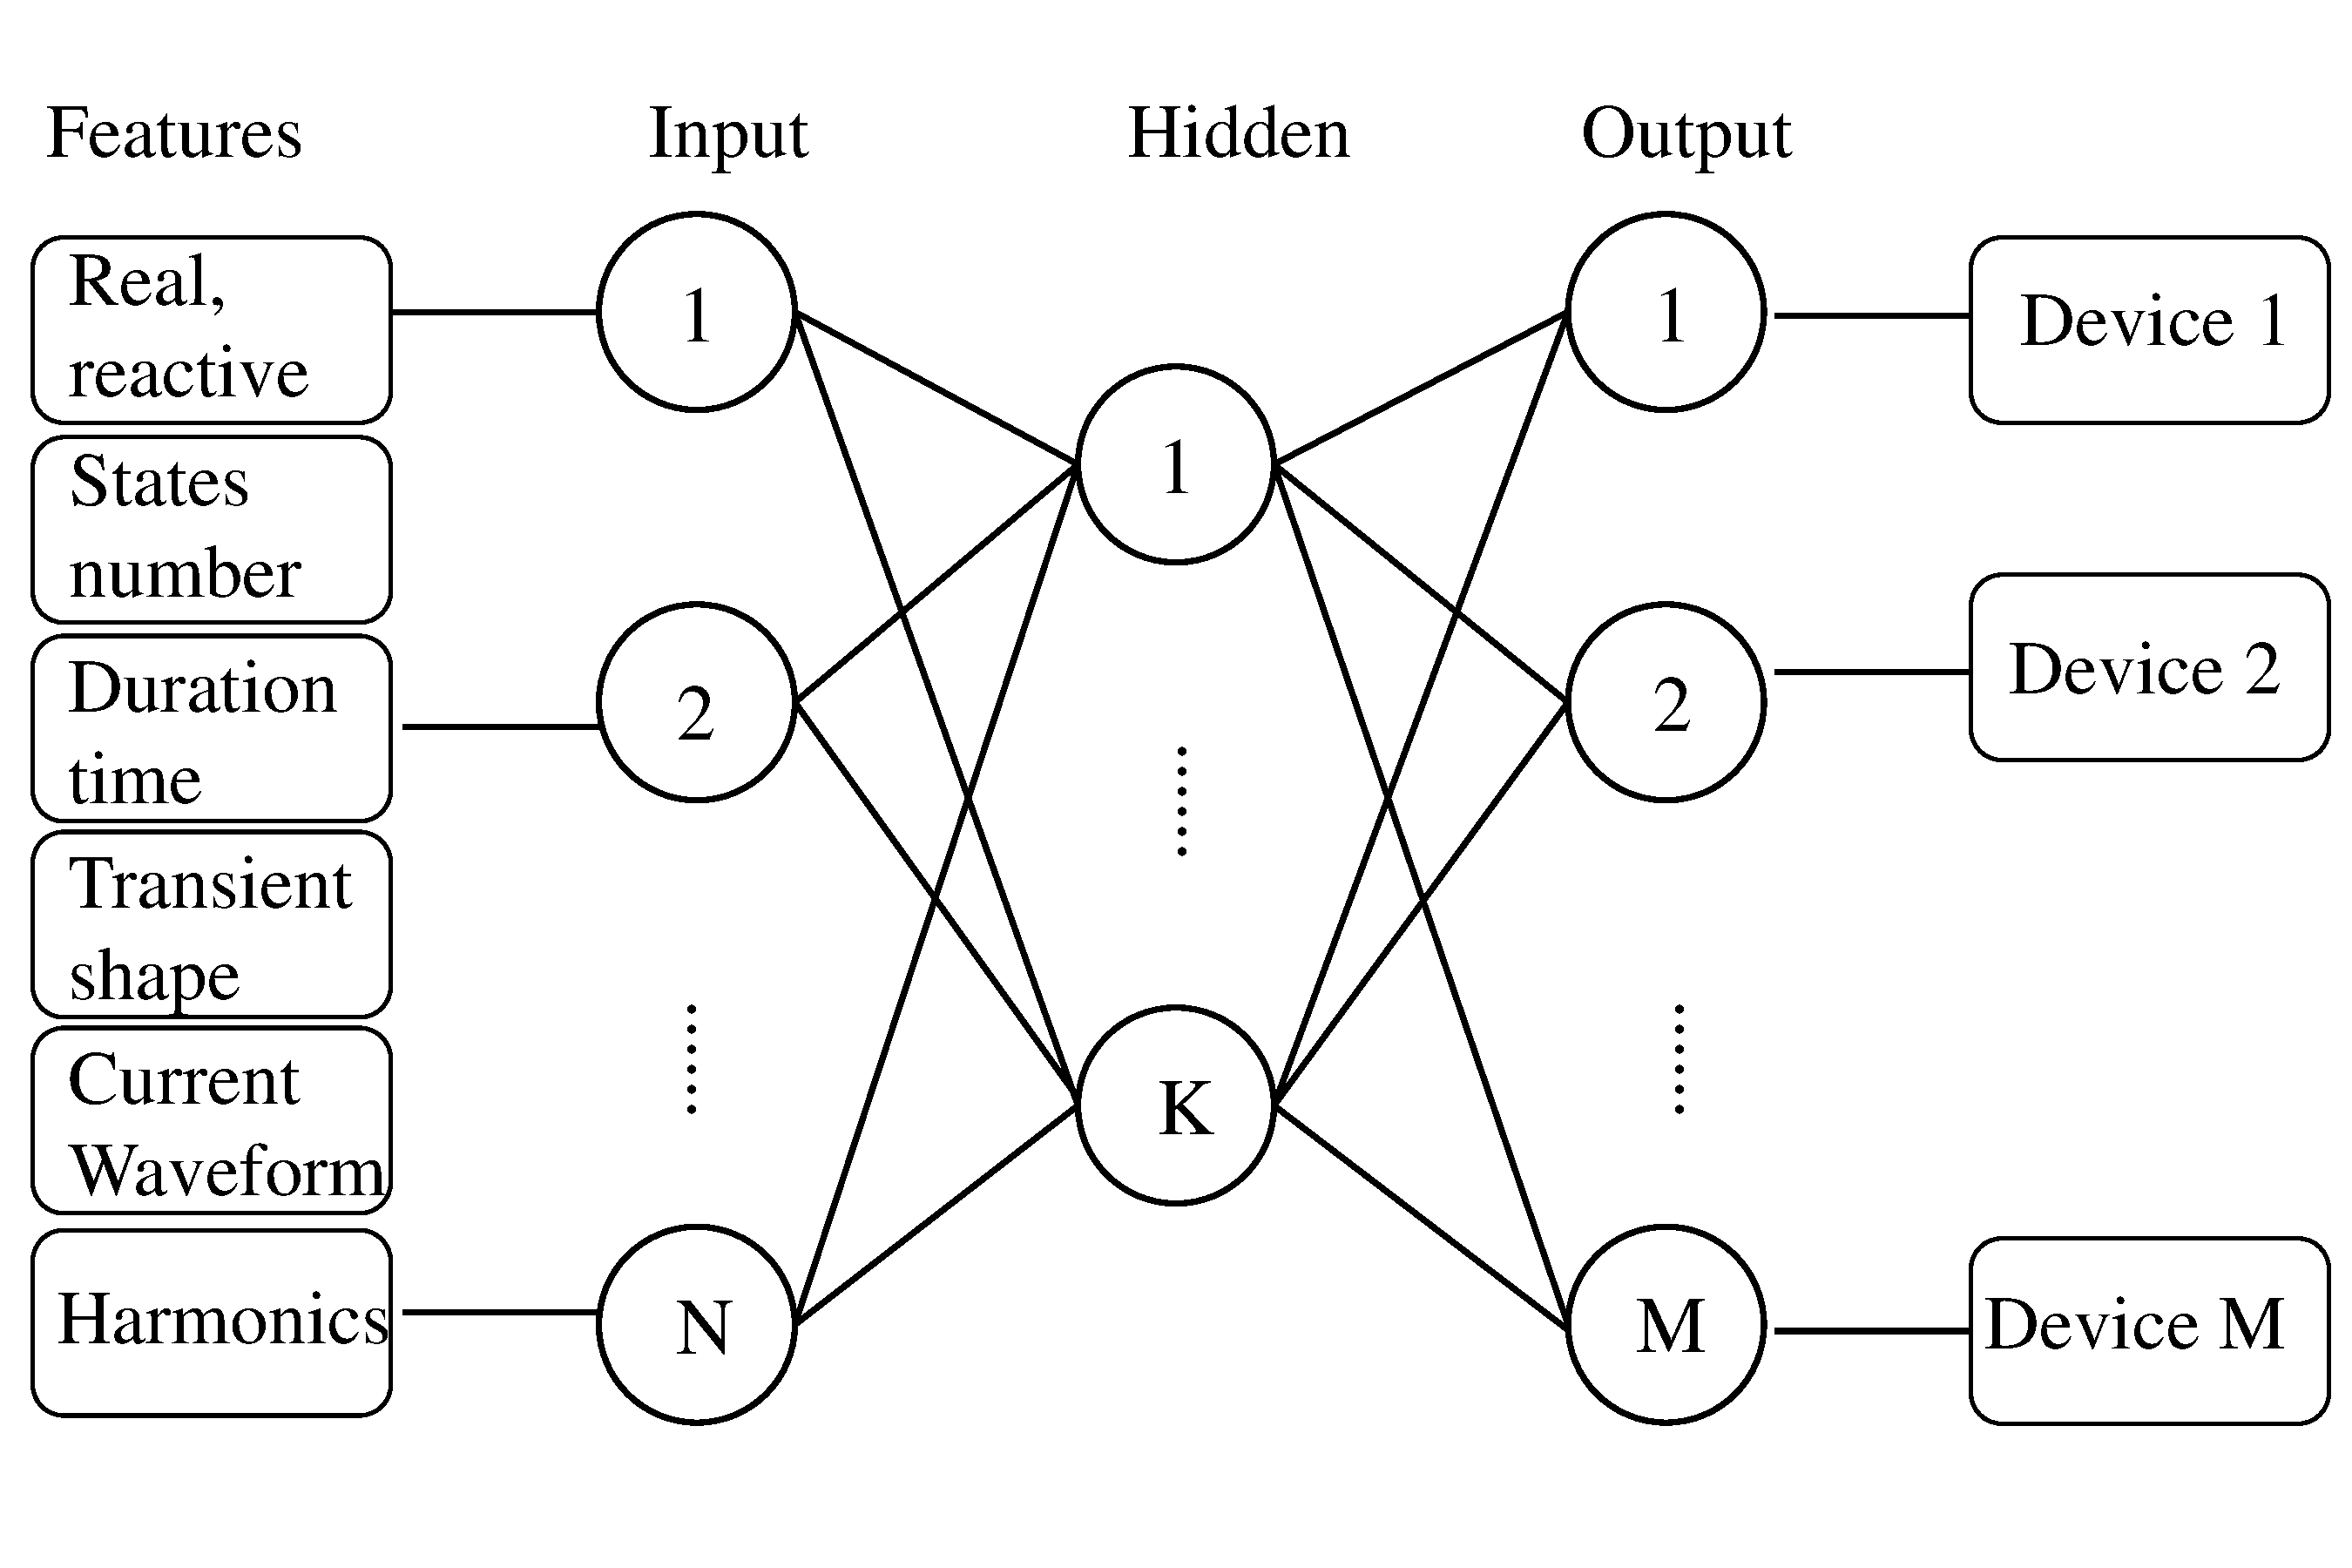
\includegraphics[width=3 in]{figs/neuralNetwork.pdf}
\caption{Neural Network Approach for Energy Disaggregation.}
\label{fig_neuralNetwork}
\end{figure}


Generally, the evaluation for a neural network-based classifier is 
to compare the relative error percentage.
%Neural network has the advantage over detect the interaction between
%the disaggregated features and ground truth
%but it works very slow.

%Several papers have adopted basic neural network for device classification. 
Roos et al. initially proposed to adopt
neural network classification for classification based on real
power and reactive power by 
transforming the aggregated data into images for processing~\cite{roos1994using}.
Next,~\cite{baranski2003nonintrusive} employs a backpropagation (BP)
neural network with the attributes of number of states,
duration time, and average energy consumption. %to identify devices.
Furthermore, 
the training stage of~\cite{duan2004neural} and~\cite{srinivasan2006neural} are based on the current waveform
and harmonics. %to extract signatures by Fourier transform thus identify devices.
The latter paper treats eight odd-numbered harmonics as a vector event feature 
for classification and chooses 16 hidden nodes.
Note that~\cite{srinivasan2006neural} compares several neural network approaches, 
namely multilayer perception (MLP), radial-basis function (RBF) network,
and support vector machine (SVM) with linear, polynomial and
RBF kernels.
The results suggest that MLP and RBF-based approaches have high classification accuracy. 

%neural network
Chang et al. extend the back propagation approach
by employing an electromagnetic transient program (EMTP) with
transient real power when devices start up~\cite{chang2008load2}. 
The transient shape is a vector event rather than a point event. 
To identify devices from aggregated data adaptively,
a window size %$\Delta t $ 
$w$
is adopted to enhance the algorithm
as an adaptive neural network. 
Initially, the differential values $dP_{transient}$ for period time %$\Delta t$ 
$w$
represent the characteristics of a class of devices. During the training process,
the time period value %$\Delta t$ 
$w$ increases by $\delta$ from $1$ to %$\Delta t$
$w$.
The $\delta$, which achieves the highest recognition accuracy, is retained.

Recently a basic adaptive neural network (ANN) applied to energy disaggregation was presented in ~\cite{liang2010load}. 
%The paper selects backpropagation ANN (BPANN) to
%train a model. 
Based on a combination of features,
such as real power, reactive power,
transient shapes, harmonics, the eigenvalue of the current waveform,
the voltage waveform, etc., 
this paper establishes a committee decision system based on 
three rules: most common occurrence (MCO), least unified residue (LUR), and
maximum-likelihood estimation (MLE), to classify devices. 
As a result, the disaggregation accuracy is high. 

%The system work flow is Figure\ref{fig_system_srinivasan2006neural}.
%In the first step, the distorted waveform generated by non-linear
%devices is transformed by Fourier analysis.
%\begin{figure}[h]
\centering
\includegraphics[width=3 in]{figs/system_srinivasan2006neural.pdf}
\caption{System for Neural Network (Courtesy:\cite{srinivasan2006neural})}
\label{fig_system_srinivasan2006neural}
\end{figure}


%Then the eight odd-numbered harmonics are extracted as vectors as
%illustrated. %in Figure\ref{fig_harmonics_srinivasan2006neural}.
%The real part and imaginary part are separated as the input of
%ANN.
%Since there are 8 devices, the output number of nodes is 8.
%The number of hidden nodes is chosen as 16.

Two variants of the basic neural network approach
have been proposed. %LVQ neural network
Reference \cite{yang2007design} classifies the transient events by way of
back propagation,  
and \cite{chang2008load} adopts learning vector quantization (LVQ) to
recognize devices. % combination with GA
Neural networks have also been combined with other approaches. For example,~\cite{chang2010newmethod} combines a multi-layer feed-forward neural network with a genetic algorithm to 
to analyze the device turn-on transient signatures. 
%%%%%%%%%%%%%%%end of neural network

%\subsubsubsection{Support vector machine}
\textbf{Support vector machines}
SVMs attack the problem using multiclass learning techniques by learning 
event features only from the training data, in contrast with unsupervised methods that learn
features from the entire dataset. 
%\manishc{that is in general true for all classifiers} \huijuanc{Yes. unsupervised disaggregation approaches learn the features from the entire dataset other than part of the dataset. I add unsupervised.}
Kernels such as the radial basis function (RBF) kernel are adopted to learn complex features like harmonics. At first, SVMs were employed to classify devices by 13 odd-order harmonic current 
and phase angles from on and off events~\cite{onoda2000applying}. 
Later, a kernel-based subspace classification (KSC) approach is used for 
events classification in SVM~\cite{onoda2000applying2}. 
%%% the following is needed or not? 10-08-2014
%The RBF kernel is introduced as Equation (\ref{eqn_rbfSubspace}). %for both KSC and SVM.
%\begin{equation}
%\label{eqn_rbfSubspace}
%k(x,y)=exp(\frac{{\lVert x-y \rVert}^2}{\sigma ^2})
%\end{equation}
%Where $x$ is the dimensional patterns,
%$y$ represents the classified devices,
%$k(x, y)$ is the kernel matrix. 
% and its $(i, j)$ element is $k(x_i, y_j)$.

SVMs were widely utilized with  noisy datasets although they
do not scale well for large data sets. 
%because 
%the size of these datasets is much larger than 
%that of AC power features and SVM has the ability to perform fast computations on
%large data sets. 
%\manishc{svm's don't scale well for large data sets}
%\huijuanc{SVM does scale for large data sets according to the following two references. "Classifying large data sets using SVMs with hierarchical clusters", "Making SVMs scalable to large data sets using hierarchical cluster indexing".}
%\huijuanc{delete the sentences related to scalability.}
An SVM was adopted by~\cite{patel2007flick}
to classify transient pulses noise from various homes.
%During processing, transient events from noise data are isolated and
%then the disaggregated events are classified into these transient events.
%The test is done for the residential buildings.
%The author figures out it could be applied to commercial buildings
%which may include more compound devices and complex noises.
In~\cite{froehlich2011disaggregated}, 
SVMs are applied to transient and continuous voltage noise data.
The noisy voltage generally produced by devices influences
the power wiring.
According to Gen Marubayashi~\cite{mambayashi1997noise},
there are three types of voltage noise:  
on-off transient noise;
steady-state line voltage noise, which is produced at $60$ Hz or
integer times of $60$ Hz (e.g. harmonics),
and steady-state continuous noise which is generated beyond
$60$ Hz.
Voltage noise data is sampled with very high frequency.
During pre-processing, the noisy recorded voltage data
is transformed by a Fourier analysis. 
Then, three to five transient voltage noise signatures are labeled
and a threshold is pre-defined.
During the training phase,
by sliding a window on the aggregated voltage noise,
a part of the data with continuous voltage noise
is extracted and compared with the pre-stored voltage noise data by measuring the
Euclidean distance.
If the distance is larger than the pre-defined
threshold, then the feature vector is exerted from
this window.
After sliding over aggregated voltage noise data,
all these feature vectors are classified
by the SVM.

In addition to their use
as a standalone classifier, SVMs are also utilized in energy disaggregation 
in combination with other approaches. 
In~\cite{nakano2007non}, 
both stand-alone SVMs and a combination of SVM and radial basis function network (RBFN)
are implemented to compare the disaggregated data with the ground truth harmonics.
%Then parameters for KSC and SVM are estimated and tested.
%The results shows that KSC performs with lower error rate
%for some devices and a bit higher error rate for other devices.
%However, the computation cost of KSC is much lower than SVM.

%Support vector machine is to find a large margin between
%two classes thus minimize the distances of each plate.
%Figure\ref{fig_svmClassifier} shows the work flow to classify ON/OFF events
%for different devices.
%\input{figs/svmClassifier.tex}

%%%%%%%%%%%%%%%%%end of SVM


%\subsubsubsection{Bayesian network}
\textbf{Bayesian networks}
A combination of SVM and dynamic Bayesian network was demonstrated in ~\cite{froehlich2011disaggregated}.
To start, a threshold value is predefined for the Euclidean distance between the new data and
basic noise data. 
Next, a window appears to determine whether the distance
exceeds the threshold. According to the Euclidean distance,
the feature vectors which characterize the devices are classified by the SVM.
Finally a dynamic Bayesian network is utilized to classify the devices based on
prior information, such as washing machines, dryers, and
HVAC.

%%%%%%%%%%%%%%%%%%%%%end of Baysian Network based

%\subsubsubsection{Rule based}
\textbf{Rule-based algorithms}
Rule-based algorithms use the different operating rules of the various devices to solve the classification problem. 
The training dataset comprises of various rules that describe the operation of a device. If a test event presents one of these rules, the device that produces that event is classified accordingly. Rule-based techniques have been primarily used in multiple-state devices. 

Closure rules with a maximal length of four were used for real power with transition states in~\cite{hampden2012closure} to classify devices.
The principle of closure rules is that
if only one device changes its state,
the baseline signature is the same as before the occurrence of the state
change.
The rules become complex for each device 
if the vector events feature is introduced. 

Rule mining is also proposed in~\cite{rollins2014using}. 
The first step is to identify candidate rules. 
For each time slot of an hour, 
a co-occurrence matrix is derived by detecting the device states. 
Through this, the time when devices are probably turned on for each 
hour of a day and each day of a week is ascertained.
In the second step, those significant rules are chosen by a 
\textit{JMeasure} (e.g., only those rules with values greater than 
0.01 are selected).

%%%%%%%%%%%%%%%%%%%%%end of Rule based

%\subsubsubsection{Naive Bayes classifier}
\textbf{Naive Bayes classifier}
%Besides aforementioned KNN,
%\cite{berges2010enhancing} also employs Gaussian Bayes Classifier
%to classify the on and off events. (???more explanation)
Algorithms that use the Naive Bayes classifier (NBC) are proposed in ~\cite{zeifman2012disaggregation} to distinguish devices. 
Based on that approach,~\cite{zeifman2013automatic} uses power and time as features to automatically disaggregate the major residential electronic devices. 

%\subsubsubsection{AdaBoost, decision tree}
\textbf{Other strategies}
Reference \cite{berges2009learning} evaluates four approaches:
k-nearest neighbor (kNN), Gaussian naive Bayes (GNB),
decision trees (DT) and multi-class AdaBoost (MultiBoost)
for high-frequency data.
Reference \cite{onoda2000applying} integrates SVM with AdaBoost to classify devices
based on odd-number harmonics.
If we suppose that in a support vector machine,
the margin $Q$ is defined as
\begin{equation}
Q= \min_{i=1,...,l}\rho(z_i,f)
\end{equation}
where
\begin{equation}
\rho(z_i,f)= y_i f(x_i)
\end{equation}
AdaBoost is used to minimize the margin
$\rho(z_i,\alpha):=\rho(z_i, f_\alpha)$ on the training set
\begin{equation}
\mathscr{G}(a)= \sum_{i=1}^l exp\{-\lVert \alpha \rVert_1 (\rho(z_i, \alpha)-\phi)\}
\end{equation}
To achieve this goal, every example $z_i$ is
given a weight $w^t(z_i)$.
Applying bootstrap on the weighted sample distribution,
we can find $\alpha_t$ to minimize $\mathscr{G}(\alpha)$, 
where $t=1,...,T$. 

%\textbf{Summary of Energy Disaggregation Classification Algorithms}

\textbf{Computational Complexity}
The computational complexity is a function of the classification approach used. 
%Kearns~\cite{kearns1990complexity} presents a comprehensive discussion on this matter. 
For training, decision trees tend to be faster than 
techniques which requires quadratic optimization such as SVMs. 
Complexity is also a function of the number and type of features.
Real power is a uni-dimensional feature and real reactive power is a two-dimensional feature. 
If harmonics, waveform and wavelet are introduced, the feature
set becomes multi-dimensional.
Neural networks have the advantage of naturally
detecting interactions between the disaggregated features and output 
time series data but training can be fraught with local minima problems.


\iffalse
\textbf{Advantages and Disadvantages of Classification Based Techniques}

The \textit{advantages} of classification based techniques are as follows:
\begin{enumerate} 
\item Compared to unsupervised learning approaches, the disaggregation accuracy is higher 
when using the same dataset as input. 
\item Compared to unsupervised learning approaches, it requires less data set to build a disaggregation model. 
%\item Classification based techniques can make use of powerful algorithms to distinguish features belonging to different devices. 
%The classification accuracy rate increases with multiple features. 
\item Compared to unsupervised learning approaches, once the model is trained, 
it has faster operation to obtain the output with input. 
%The test phase works very fast since each test instance needs to be compared against the pre-computed model.
\end{enumerate}

The \textit{disadvantages} of classification based techniques are: \manishc{I
  would think the main disadvantage of supervised methods is that labelled
  data is hard to get}\huijuanc{updated.}
\begin{enumerate}
\item The labelled data of each device is hard to get because the cost would be very high if installing meters to monitor each device. 
%\item The classification based techniques rely on the accuracy of  the extracted features of each device. 
%However these features  are hard to access in practice because of the meters that capture these measurements have a very high installation cost.
\end{enumerate}

\fi
%%%%%%%%%%%%%%%%%%%%%%%%%%%%%%%%%%%%%%%%%%%%%%%%%%%%%%%%%%%%%%%%%%%%%%%%%%%%%%%%%%%%%%%%%%%%%%%%%%%%%%%%%%%%%%

\subsubsection{Nearest Neighbor-Based}
Several energy disaggregation algorithms have been designed using nearest neighbor (NN) techniques. These techniques generally make the the following assumption:

Assumption: \textit{Feature instances from the same device occur in dense neighborhoods, 
whereas different device feature instances occur further away from their nearest neighbors.}

For all these NN techniques, obviously, a distance or similarity measure between two instances 
must be defined in order to perform device classification. 
There are different ways to compute the distance (or similarity) between two data instances.
For disaggregation of single feature, viz. point event or vector event, 
Euclidean distance is a common choice~\cite{gupta2010electrisense}.
For disaggregation of multiple features, that is, several point events or vector events, 
the distance between two instances is computed as the Euclidian distance across the dimensions of the vector event as in~\cite{shaw2000PhdThesis}. 

Nearest neighbor-based energy disaggregation techniques can be grouped into 
two categories: 
\begin{enumerate}
\item Techniques that use the distance of a data instance to its $k^{th}$ nearest neighbor 
as the measurement. 
\item Techniques that use the relative density of each data instance as the measurement. 
\end{enumerate}

%\subsubsubsection{Using distance to $k^{th}$ nearest neighbor}
\textbf{Using distance to $k^{th}$ nearest neighbor - }
The basic nearest neighbor technique has been applied to detect 
multiple features such as transient power shape~\cite{shaw2000PhdThesis,lee2005estimation,berges2009learning,berges2010enhancing}.

%makes use of
%K-Nearest Neighbor (K=1)
%to classify the ON/OFF events created by all devices with features real power, 
%reactive power, harmonics and other features. 
%In the experiment, refrigerator is tested by comparing with the plug-level
%data which is installed to monitor the monitor.
%Event classification error rate is the evaluation metric.
%The experimental results show that other two devices with similar power levels of
%refrigerator increase the predicting error rate of events produced
%by refrigerator.



%The comparison of this approach just makes use of the
%Euclidean distance to measure the similarity of
%identify events with the pre-defined spectral envelop
%of device.
Reference \cite{shaw2000PhdThesis} describes how transient shapes of power consumed by devices over time are discovered.
Transient shapes that are exemplary of each device are summarized and recorded 
in the form of real and reactive power P-Q by analyzing the data from each device. 
%The P-Q power of the aggregated data is discrete.
A pre-defined window size of 100 data points is used.
As the aggregated data flow is taken into account, consequently 
the data points in each window are compared with 
the pre-stored exemplar. 
If the Euclidean distance is smaller than the pre-defined threshold, 
an event is said to have occurred in this window, and 
it matches a pre-stored exemplar. 
%Hence, this event should be grouped into the corresponding device's attribute set. 
Based on this grouping,~\cite{shaw2008nonintrusive} decomposes the 
real power transient shape into two vectors; a shape vector and a time vector, 
rather than setting the whole transient shape as a device feature. 
Figure~\ref{fig_kNN} depicts an exemplar
with two shape vectors, $s_1$ and $s_2$.
\begin{figure*}[h]
%\centering{
%    \begin{tabular}{cc}	
	
%    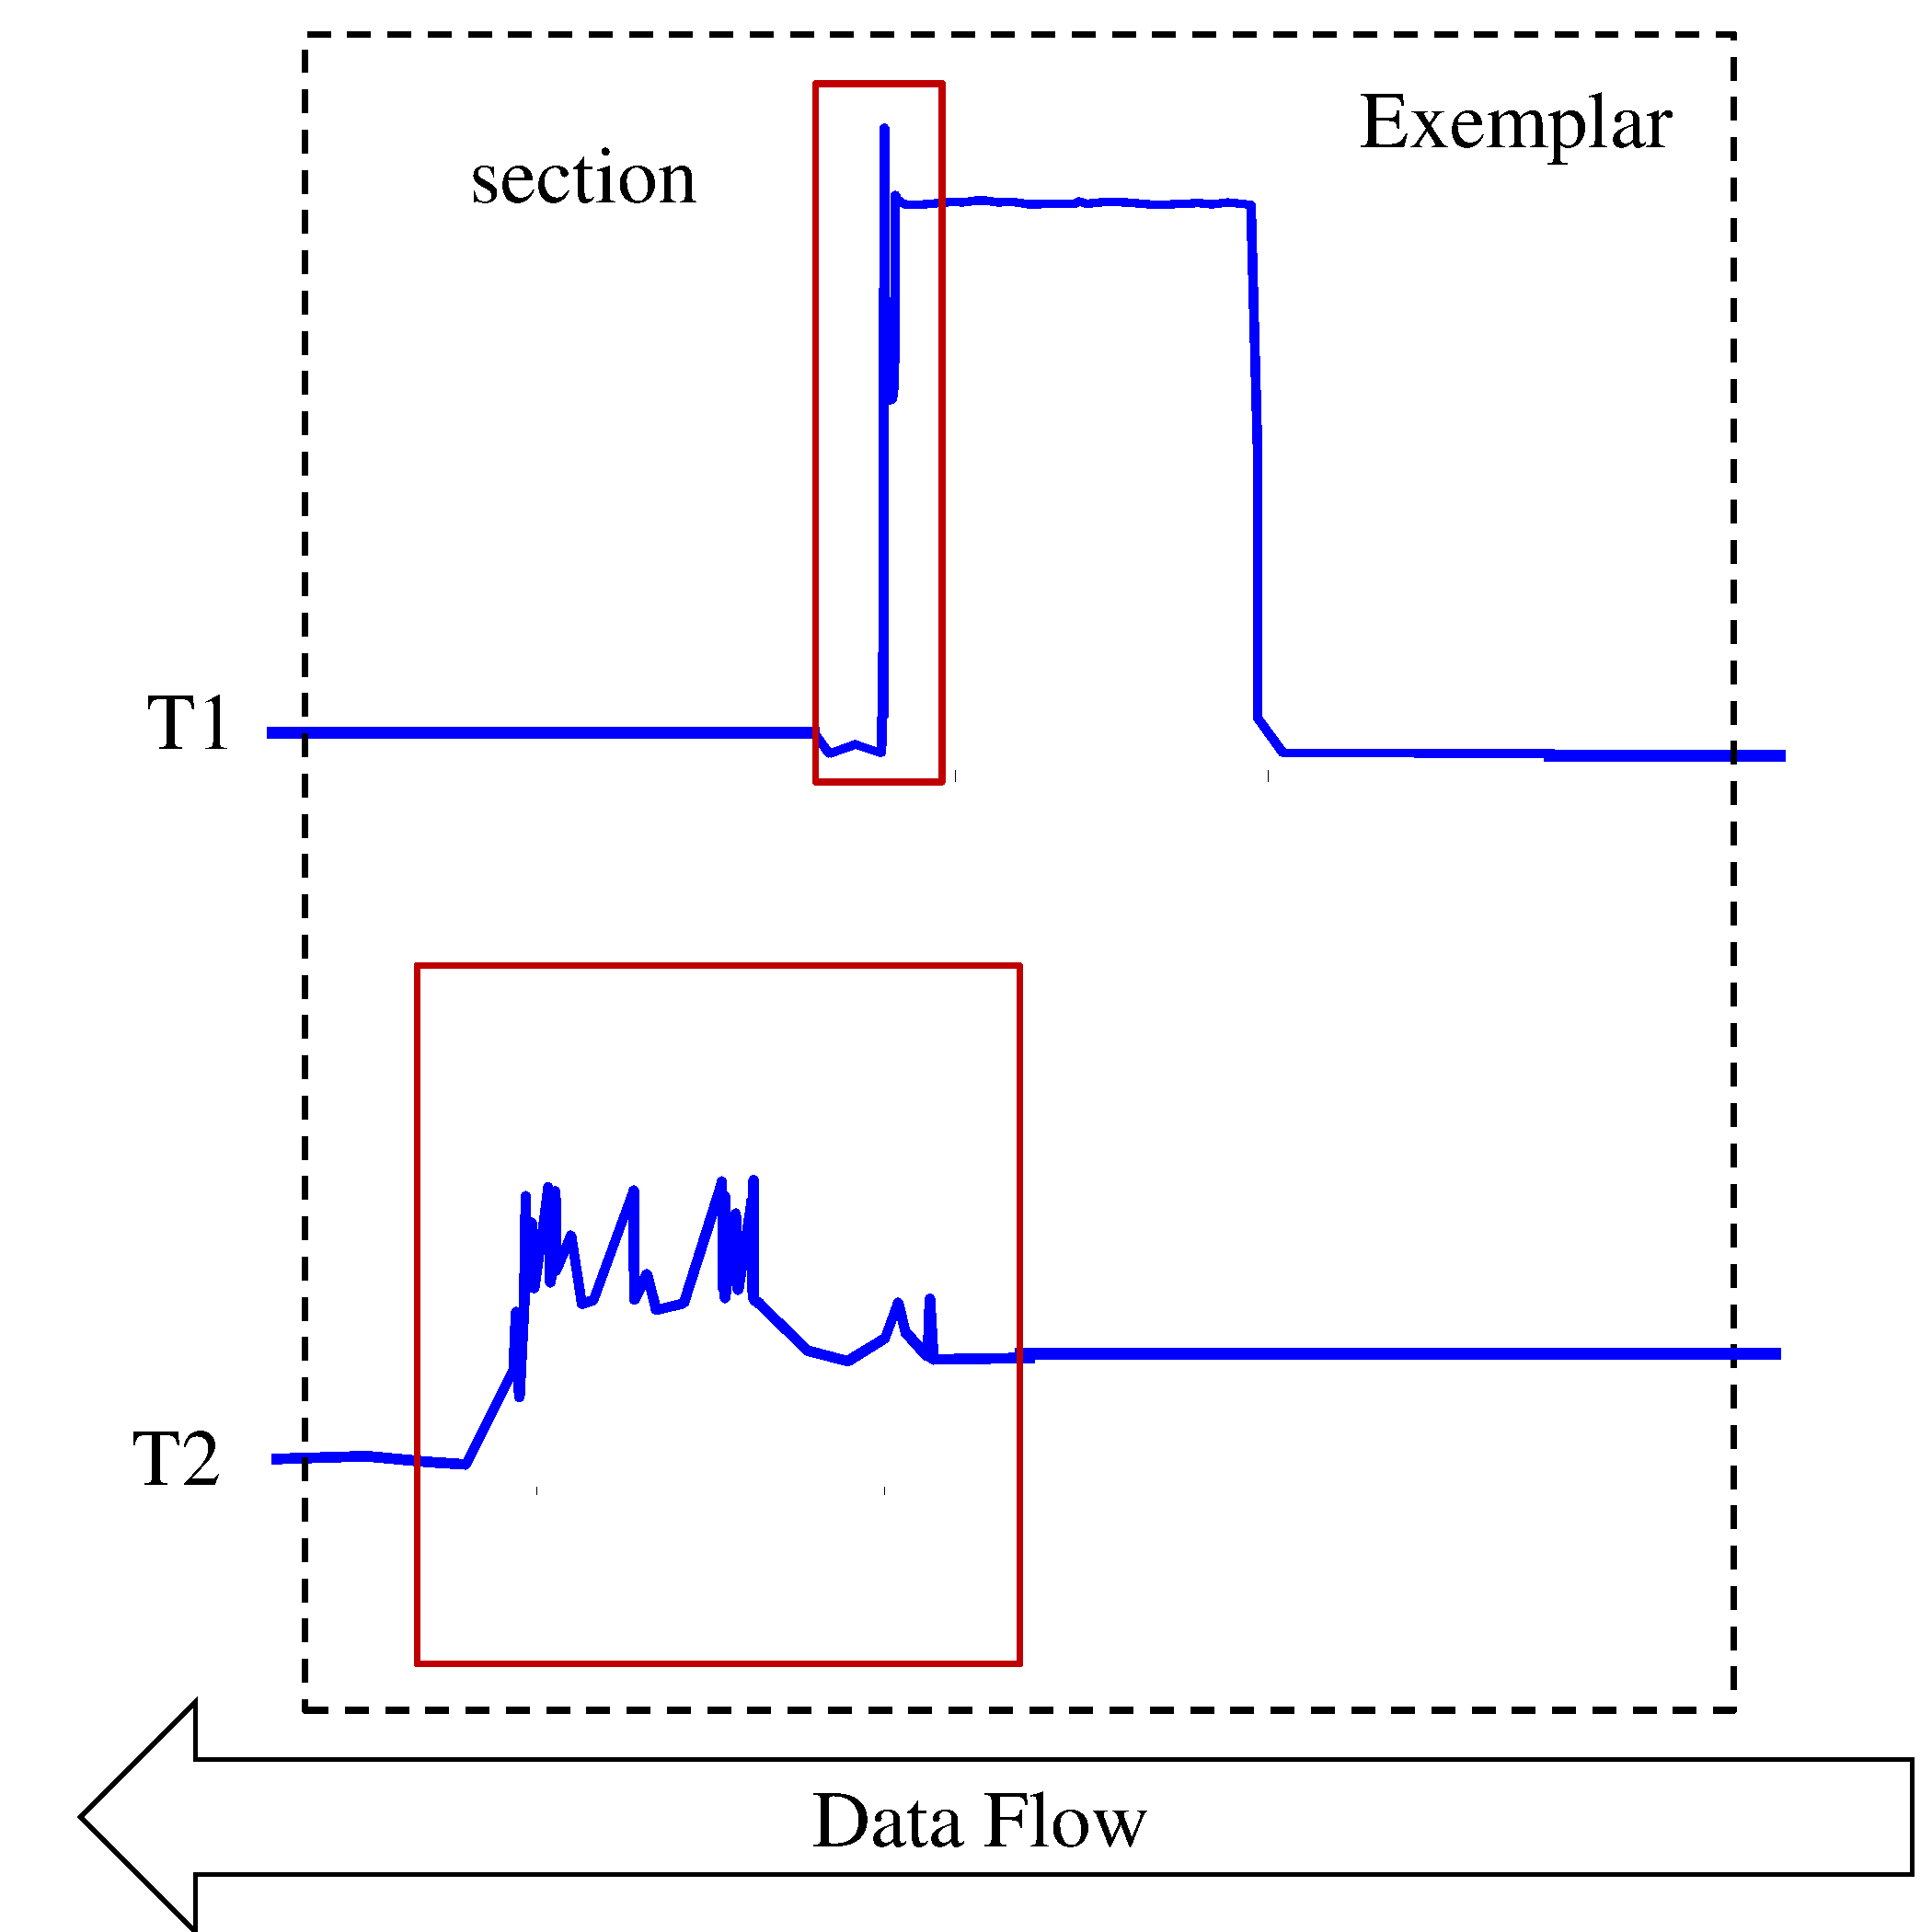
\includegraphics[width=0.4\textwidth,height=0.3\textheight]{figs/shaw2000_transientClassifier.pdf} \hspace{1em}&
%    \includegraphics[width=0.4\textwidth,height=0.3\textheight]{figs/shaw2008non_transient.pdf} \tabularnewline
%    (a) & (b)\tabularnewline
%    \end{tabular}
%    }
    \centering
    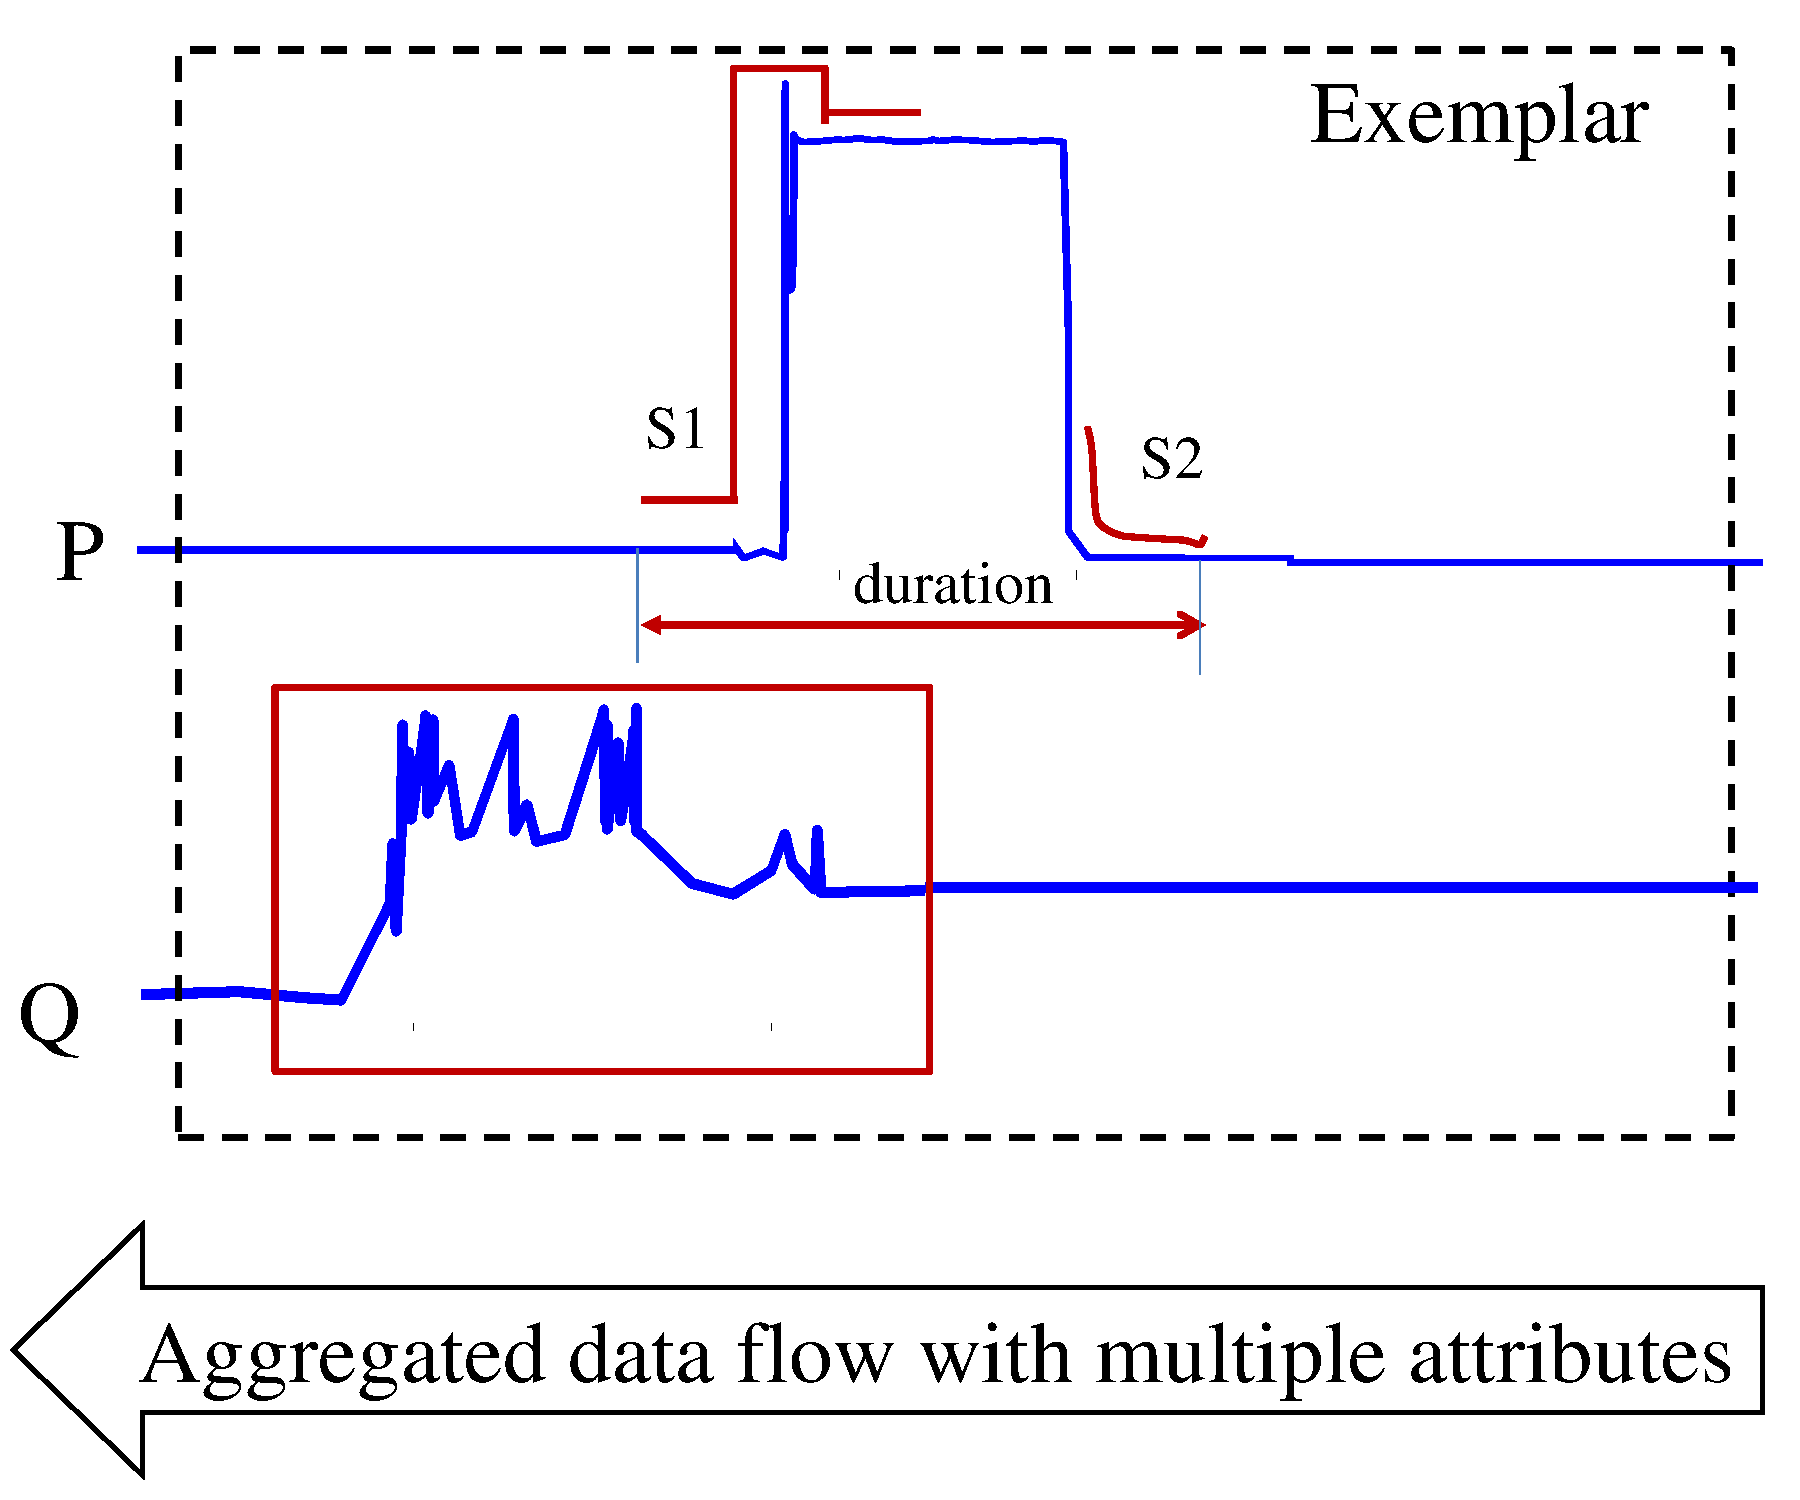
\includegraphics[width=3 in]{figs/kNN.pdf}
	\caption{Transient Shape Decomposition and KNN Search}
    \label{fig_kNN}
\end{figure*}


To identify which device the disaggregate signature belongs to,
it is necessary to compare the signature with an exemplar
by the least square criteria.
After that, a similar exemplar comparison approach is applied to identify the devices. 
The advantage of real power shape decomposition is that 
 when comparing the transient shapes,
only some characteristic parts are needed
rather than the entire transient shape in the data.
This helps cut computational cost for the exemplar comparison phase. 
Although this paper doesn't mention the KNN algorithm explicitly,
the description in this paper exactly matches the methods used in KNN algorithms to search for closest shapes.

A variant of the KNN approach measures the Euclidean distance with inverse weighting~\cite{gupta2010electrisense}. 
The variant KNN is employed to identify devices
with switch-mode power supplies (SMPS) that have power line noise features. 
These power baseline noise signatures of each device are stored as vectors, 
and 8dB is set as the power threshold above the noise baseline.
In order to classify events from aggregated data into 25 noise events corresponding to 
25 devices, a window is set to calculate the difference vector. 
After a new event is added on a particular power line,
the distance between the vector of the newly-added event and 
the baseline noise vector is calculated. 
If there is a peak above the pre-defined threshold, 
a Gaussian function is applied to calculate 
the mean, standard deviation of the difference vector. 

%\cite{berges2009learning} tests with four approaches,
%K-Nearest Neighbor, Gaussian Naive Bayes(GNB),
%Decision Trees(DT) and Multiclass Adaboost(MultiBoost).

Another variant KNN, discussed in~\cite{lee2005estimation},  
identifies variable speed devices (VSDs).
It builds a table to store
the real power, reactive power and harmonics for each device.
Then the signatures extracted from the aggregated power
are compared with the stored features.
The disaggregated signature is assigned to the device,
whose feature is most similar to the stored feature.
Since this process essentially replicates the K-nearest neighbor mechanism,
~\cite{lee2005estimation} is classified into the KNN category.


%\subsubsubsection{Using relative density}
\textbf{Using relative density}
Techniques that estimate the density of the neighborhood of each data instance are also popular in device classification.
The classification is based on whether the instance lies in a neighborhood of high or low density.  If an instance lies in a neighborhood with high density, it is declared to be in the device group corresponding to that neighborhood. 
%On the other hand, an instance that lies in a low density neighborhood does not belong to the %device's featuredgroup.  

Given an instance as a center, circles with varying radii are drawn around it.
The distance to its $k^{th}$ nearest neighbor is equivalent 
to the radius of a hyper-sphere. 
In a probability density graph, 
this distance represents the inverse of 
the dataset's density~\cite{kolter2010redd}.
A real power probability density function is used 
as a feature to classify two-state devices in~\cite{zeifman2011viterbi}.
The number of the device is indexed by the power, 
as shown in Figure~\ref{fig_realPowerPDF}.
\begin{figure}[h]
\centering
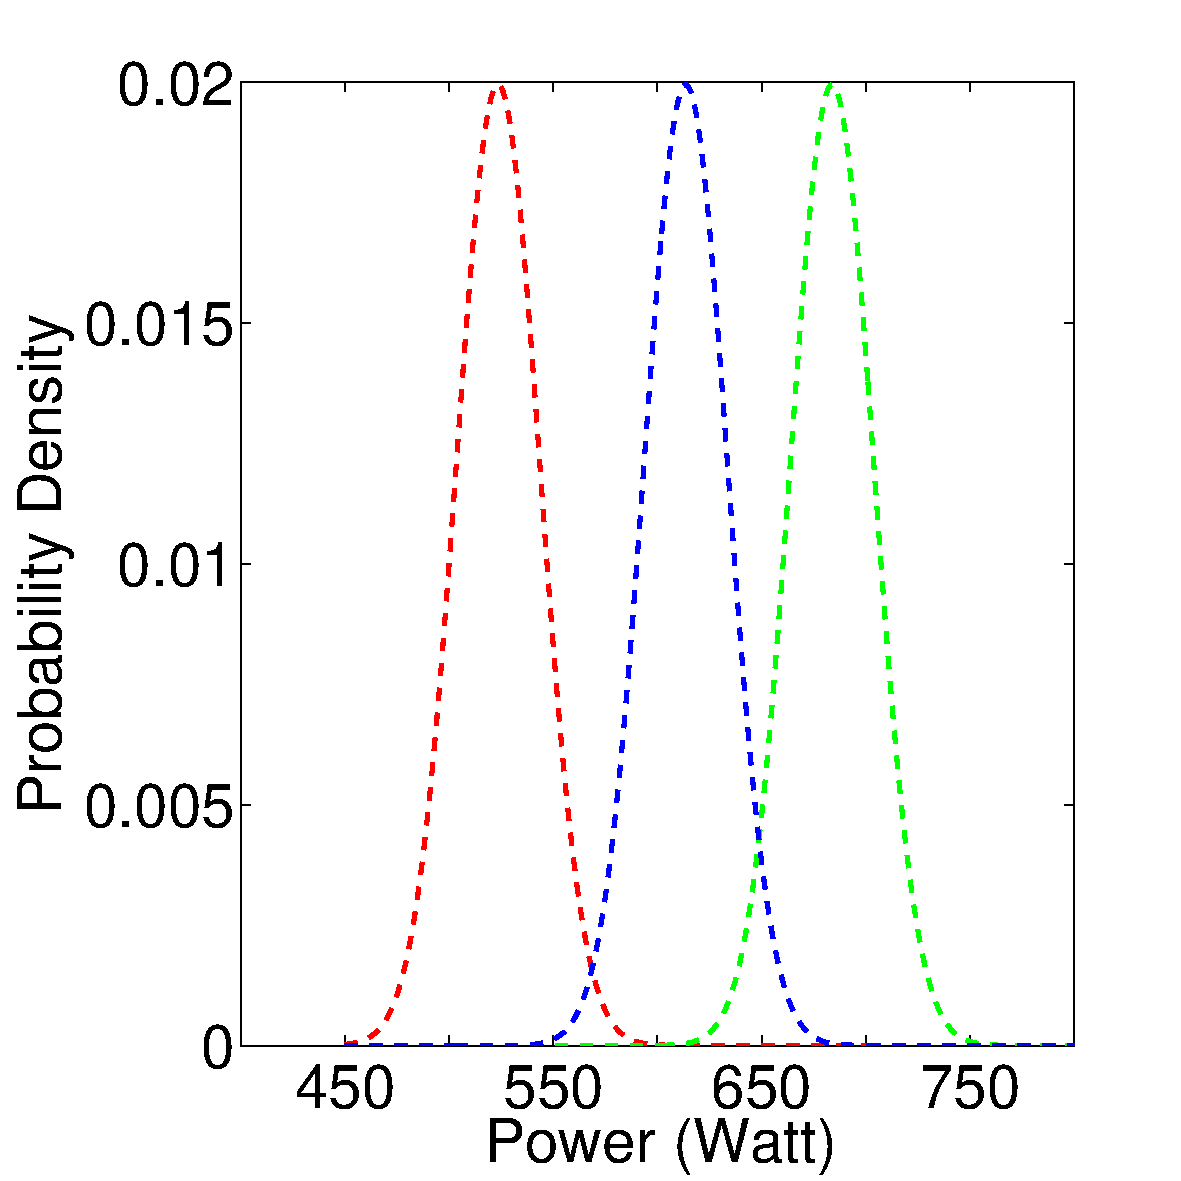
\includegraphics[width=3in]{figs/pdfRedd.pdf}
\caption{Probability density functions of three appliances neighboring by power draw.}
\label{fig_realPowerPDF}
\end{figure}


In the training step, 
the real power probability density function of each device 
is obtained by analyzing each device's actual power consumption. 
In the classifying phase,
the negative values are first clustered, and the $mth$ cluster
represents device $m$.
Next, the positive values are clustered to match the negative clusters.
The real-power probability density function is used to match the negative values to their corresponding positive counterparts.

%\textbf{Summary of Energy Disaggregation Nearest Neighbor Algorithms}

\textbf{Computational Complexity}
A drawback of basic nearest-neighbor approaches is that the 
time complexity is $O(N^2)$.
%because all the instances are compared pairwise.
If multiple attributes are employed with window size $w$ instead of only 
real power, the computation cost is even higher than $O(N^2)$. 

\textbf{Advantages and Disadvantages of Nearest Neighbor Based Techniques}

The \textit{advantage} of nearest-neighbor based devices classification is 
that it's straight-forward and primarily requires a proper distance measure for the given features. 

The \textit{disadvantages} of nearest-neighbor based devices classification techniques are as follows:
\begin{enumerate}
\item The computational complexity at the test stage is high, 
especially for the high-frequency data with vector features. 
The algorithms require comparison of the aggregated data of all device features at each window to obtain the nearest instance. 
\item When multiple features are applied, defining the measure of distance becomes challenging because different features have different units of distance.
\end{enumerate}

%%%%%%%%%%%%%%%%%%%%%%%%%%%%%%%%%%%%%%%%%%%%%%%%%%%%%%%%%%%%%%%%%%%%%%%%%%%%%%%%%%%%%%%%%%%%%%%%%%%%%%%%%%%%%%
\subsubsection{Statistical Model-Based}
Statistical approaches to devices classification assume that \textit{a device instance belongs to a high probability region of 
a stochastic model, while not belonging to a region at low probability.}

Statistical techniques fit a stochastic model given the event features from all devices. 
A statistical inference test is applied to determine whether an 
unseen event extracted from the aggregated data belongs to this model. 
Instances with low probability generated from the learnt model 
are declared as wrong event classification. 
Both parametric and non-parametric techniques are used to fit a statistical model. 
Parametric techniques assume that the underlying distribution of 
events are known whereas non-parametric techniques posits that this 
underlying distribution is unknown. 


%\subsubsubsection{Parametric models}
\textbf{Parametric models}
%Goodness-of-fit
As discussed above, parametric techniques assume that 
the device's features follow a parametric distribution 
with parameter $\theta$ and probability density function $F(y,\theta)$, 
where $y$ is the observation. 
The score of a test instance is the inverse of the probability density function. 
%(Ziefman paper??probability density function)

An alternate approach is the hypothesis test.
The $null$ hypothesis ($H_0$) is that a test instance $x$ has been generated 
using the estimated distribution with $\theta$. 
If the statistical test rejects $H_0$, 
$x$ is declared to not belong to this device's distribution. 

Reference \cite{jin2011robust,jin2011time} use goodness-of-fit (GOF) chi-squared
to detect the transient events generated by
the first harmonics of power consumption.
GOF utilizes the hypothesis approach.
At first, a change point in time-series data is detected.
%\cite{jin2011robust} has good definition in window definition
%some idea: Bayesian to find the events detection instead of Chi-square tests
For $i$ independent and identically distributed (iid) data points $y_t,t=1,2,...,T$
are drawn from a distribution $G(y)$ and the supposed distribution $F(y)$.
The binary hypothesis testing problem is defined as
\begin{eqnarray}
H_1: G(y) \ne F(y) \\
H_0: G(y) = F(y)
\end{eqnarray}
After this the $\chi^2$ test for goodness-of-fit(GOF) is defined. 
If the $\chi^2$ hypothesis condition is satisfied, 
then the feature is classified into the supposed device. 

%%%%%% such long discussion is not needed. 10-08-2014 Huijuan
%\begin{equation}
%\mathscr{l}_{GOF} = \sum_{i=1}^{n} \frac{(y_i - x_i)^2}{x_i}
%\end{equation}
%When the condition in Equation (\ref{eq_chisquare}) is satisfied,
%e.g. with $100(1-\alpha)\%$ confidence interval,
%$H_0$ hypothesis is rejected.
%\begin{equation}
%\label{eq_chisquare}
%\mathscr{l}_{GOF} > \chi_{\alpha,n-1}^2
%\end{equation}
%This means this feature can be classified into the supposed device.
%%%%%%%%%%% 10-08-2014 Huijuan

A generalized likelihood ratio is applied in~\cite{anderson2012event}, ~\cite{berges2011user} and ~\cite{luo2002monitoring}. 
These papers use the generalized likelihood ratio to classify
the events generated by different devices.

First, the mean power value before and after a time $t$ is calculated. 
Given the aggregated data,  
the log ratio of probability distribution before and after each event 
is calculated as follows. 
\begin{equation}
R= \prod_{t=j}^{k}\frac{F_{u_t}(y_t)}{F_{u_{t-1}}(y_t)}
\end{equation}
where $y_t$ is the sampled variable at time $t$, 
$u_t$ is the mean value of the sampled sequence at time $t$, 
and $F_{u}(y_t)$ is the probability density function of the sampled sequence 
$y_t(t=j...k)$ about the mean value $u$. 
The greater the probability, the greater the chance the data points belong 
to a specified device. 

%\subsubsubsection{Non-parametric models}
\textbf{Non-parametric models}
The non-parametric techniques in this category do not 
define a  prior assumption such as smoothness of density.
The model is driven directly by the data.

A hierarchical probabilistic model is proposed in~\cite{wang2013heirarchical}.
It aims to find devices with multiple states. 
It utilizes the device-on distribution and real power features. 
In the hierarchical probabilistic model, a three-layered model is applied. 
The first layer is a feature layer, the second layer is a state layer, 
and the last layer is a consumption layer. 
The objective function estimates the maximum a posteriori (MAP) 
probability that an event belongs to a device. 
Since the computation cost is high, it 
utilizes a heuristic approach. 

% not sure what spare coding belongs
%\textbf{Summary of Energy Disaggregation Statistical Algorithms}

\textbf{Computational Complexity}
The computational complexity of statistical techniques 
depends on the nature of the fitted statistical model.
Fitting single parametric distributions from the exponential family, 
e.g. Gaussian, is linear in data size as well as number of attributes. 
Fitting complex distributions such as Gamma distribution~\cite{kim2011unsupervised} 
using iterative 
estimation techniques such as expectation maximization (EM) are 
typically linear per iteration, though they might be slow 
in converging depending on the problem and convergence criterion. 

\textbf{Advantages and Disadvantages of Statistical Model-Based Techniques}
The \textit{advantage} of statistical techniques is :
\begin{enumerate}
\item If the assumption regarding the underlying data distribution 
holds true, statistical techniques provide a sound device classification. 
\end{enumerate}
The \textit{disadvantages} of statistical techniques are:
\begin{enumerate}
\item The device classification primarily relies on the assumption 
that the data is generated from a particular distribution, but this assumption often does not hold true, especially for multiple-state 
devices. 
\item Even if the distribution assumption is true, 
there are several hypothesis tests for devices classification,  
and it is difficult to choose a proper hypothesis test when dealing with a complex distribution. 
\end{enumerate}
%%%%%%%%%%%%%%%%%%%%%%%%%%%%%%%%%%%%%%%%%%%%%%%%%%

\subsubsection{Optimization-Based}
There are several techniques that cast device classification as an optimization problem. In this formulation, energy disaggregation is specified as an objective function that minimizes the error.

% or maximize the likelihood function of ??

%The detailed algorithm is describe in Figure\ref{fig_DDSC_kolter2010sparse}
%\begin{figure}[ht]
%\centering
%\includegraphics[width=5in]{figs/DDSC_kolter2010sparse}
%\caption{Discriminative Disaggregation Sparse Coding:\cite{kolter2010sparse})}
%\label{fig_DDSC_kolter2010sparse}
%\end{figure}
%\begin{equation}
%\tilde{E}_{reg}(X_{1:k},B_{1:k},\tilde{B}_{1:k}) \equiv \sum_{i=1}^{k}()
%\end{equation}

%\subsubsubsection{Dynamic programming}
\textbf{Dynamic programming}

Reference \cite{baranski2004detecting} utillizes mathematical dynamic programming
with the genetic algorithm to find the multiple-state device that are represented as finite state machines (FSM).
%A  variant solution for dynamic programmining is to solve with 
%heuristic solutins such as genetic programmining.
In this paper, 
the genetic algorithm is integrated with clustering and 
dynamic programming as an approach to solve the devices classification 
problem.% in \cite{baranski2004genetic}. 
The whole procedure is broken down into four steps. 
In the initial step, a finite state machine is used to describe the real power change events for each device.
The real power change events are detected from the aggregated data. 
All the on and off events shown in the time series 
are represented as $\Delta y_t =y_t - y_{t-1}$.
In the second step, fuzzy clustering is used to cluster all the 
detected real power change events. 
In the third step, all finite state machines are 
created by a genetic algorithm. 
%(input?output?)
At the final stage, dynamic programming is applied to 
discover the shortest path in those finite state machines. 

The qualification of disaggregated finite state machines
is evaluated as follows. 
Shannons entropy is introduced to compare 
the shortest path 
to the pre-stored path of finite state machines.
Assume a shortest path $\Gamma_l={S_{l1},...,S_{lk}}$
and a device's finite state machine path $\Gamma_m={S_{m1},...,S_{mk}}$, 
the Shannon entropy is calculated as Equation (\ref{eq_shannon}).
\begin{equation}
Q_l=  - \sum_i \Delta e_i log|\Delta e_i|
\label{eq_shannon}
\end{equation}
and
where 
$\Delta e_i = |\frac{\sigma_i(\Gamma_l)-\sigma_i(\Gamma_m) }{\sigma_i(\Gamma_m)}|+e_0 $
and $\sigma_i$ represents either ON duration between state changes or real power standard deviation of
the state $S_i$.
The shortest path with least entropy belongs to device $m$ which has the characteristics of 
state machine $\Gamma_m$.
This genetic programming based optimization approach 
is applied to the features of three current and voltage features. 
%For instance, power levels such as (150W, 50W, -200W) can be found 
%in the aggregated data. 
%Genetic programming reduces the number of finite state machines.

In~\cite{chang2010newmethod},
genetic programming is integrated with the neural network
to identify devices. In~\cite{vogiatzis2013real} clustering is integrated with finite state machine 
and dynamic programming to disaggregate the devices in real time with low cost.
%the cost computation?

%\subsubsubsection{Dynamic model}
\textbf{Dynamic model}
\cite{dong2013dynamical} assumes that each device has an input and an output then 
applies a dynamic approach to simulate the disaggregation process. 
Each device is represented as linear time-variant state-space model over the 
entire time series. 
The problem is formalized as Equation~\eqref{eqn_dynmodel}.
\begin{equation}
\label{eqn_dynmodel}
\begin{aligned}
\argmin_{\hat{y},x} \mathcal{L}(\hat{y},y) + g(x) \\
s.t. \hat{y_m} = h_m(x_m)\\
\hat{y}=\sum_{m=1}^{M} \hat{y_m}
\end{aligned}
\end{equation}
where $m\in{1,...,M}$, $M$ is the number of devices, $x_m$ is the input to the device $m$, and 
$h_m$ is a function which denotes the underlying dynamics. 
To estimate $x[\cdot]$, blind system identification techniques~\cite{abed1997blind} are used. 
%integer programming
%\subsubsubsection{Integer programming}

\textbf{Integer programming}
Integer programming~\cite{suzuki2008nonintrusive} is applied
to the current waveform in a supervised learning setting.
Each device's waveform which spans $T$, where $T$ is 1/50 or 1/60 seconds,   
is stored in the database,
then a disaggregation process moves on to identify the
devices according to the pre-stored current waveform.
This paper supposes there are $N$ kinds of devices, 
and there are $C_n$ appliances for each kind of device. 

Let us suppose there is an aggregated load \textit{current} $y$,
\begin{equation}
y_t= \sum_{m=1}^{M}c_m(s_m)x_{t}^{(m)}+\epsilon
\end{equation}
where $c_m \in \{0,...,C_m\}$ is integer variable for $m\in\{1,...,M\}$, 
$t \in \{1,..., T\}$, 
$x_{t}^{(m)}$ represents the current of  $m$ kinds of devices at time $t$, 
$M$ denotes the number of device types, 
$c_m(s_m)$ is the operation states of one appliance $c_m$ belong to kind $m$ if 
eace device has only one operating mode. 
%If each device has multiple operating modes $S_m$, 

$\epsilon$ represents noise. 
To estimate $c_m$ from the aggregated $y_t$, 
this problem is abstracted as an integer
quadratic programming problem
\begin{equation}
\min \sum_{t=0}^{T-1}(y_t- \sum_{m=1}^{M}c_m(s)x_{t}^{(m)})^2
\end{equation}
subject to
\begin{displaymath}
c_m \in \mathcal{Z}, 0 \leq c_m \leq C_m, \forall m \in \{1,...,M \}.
\end{displaymath}

%viberbi algorith
%The problem of positive and negative real power matching is 
%that devices with close real  power levels would overlap. 
%That is, device $i$ overlap may be mixed with device $i-1$ and $i+1$ as illustrated 
%in Figure\ref{fig_realPowerPDF}.

%In order to separate devices from the PDF,
%only the PDF relationship of $(i-1, i)$ and
%$(i, i+1)$ need to be considered.
%The Viterbi-type algorithm can greatly
%decrease the computational cost compared
%to brute-force Viterbi algorithm.
%Its computation complexity is linear
%to the number of devices.

%The on duration of each device and its 
%It applies viterbi algorithm to
%devices with several two-states with Probability Density Function of
%the real power.

%\subsubsubsection{Viterbi algorithm}
\textbf{Viterbi algorithm}
Another paper~\cite{zeifman2012disaggregation} 
employs real power probability density functions (PDFs) by a conjunction of semi-Markov and Viterbi-type algorithms to distinguish devices. % without training.
%Figure\ref{fig_pdf_ziefman2012} shows a device with many power levels which
%overlap with five devices.
%\begin{figure}[ht]
%\centering
%\includegraphics[width=3in]{figs/pdf_ziefman2012.png}
%\caption{Possible PDFs of power draw of appliances i and its neighbors (courtesy: \cite{zeifman2012disaggregation})}
%\label{fig_pdf_ziefman2012}
%\end{figure}
The standard Viterbi algorithm is used to maximize the likelihood of power
draws of appliance $m$ and its neighbors. 

%appliance $i$ to
%be turned on or off on the power change ΔP can be expressed
%through the probability density function (PDF), conditional for
%a given appliance.

\begin{equation}
\{\hat{S}_t \} = {argmax}_{s_t}[\{S_t\}|\{\omega_t\}]
\end{equation}
where $\{S_t\}$ is the state sequence and
$\{\omega_t\}$ is the transition observations.

The Viterbi algorithm adopts a similar approach to the one mentioned in~\cite{baranski2004genetic}.
The difference of this method is that they introduce the probability density function of real power of each device. 

%\subsubsubsection{Sparse coding}
\textbf{Sparse coding}
Reference \cite{kolter2010sparse} introduces non-negative sparse coding to solve the energy disaggregation problem. 
It is composed of three major steps. 
The first step is the sparse-coding pre-training step, which aims to 
model each source using non-negative sparse coding by solving 
Equation (\ref{eq_sparsepretraining}).
\begin{equation}
\min_{A_m\geq0,B_m\geq0}\frac{1}{2}\lVert X_m- B_mA_m\rVert_F^2 + \lambda\sum_{p=1,q=1}^{r,s}E(A_m)_{pq}
%subject \qquad to \qquad \lVert B_i^{(j)} \rVert_2 \leq 1, j=1,...,n
\label{eq_sparsepretraining}
\end{equation}
such that $A_m \in R_{+}^{r\times s} $ and
 $B_m \in R_{+}^{T\times r}$, 
where 
$X_m \in R^{T \times s}$ represent the $s$th power level associated with device $m$. 
The columns of $B_m$ represent $r$ basic functions corresponding to features, 
the columns of $A_m$ represent the activation, i.e. sparse codes of these basic functions set, 
$\lambda$ represents the sparseness degree, 
and $F$ denotes the Frobenius norm. 
This optimization is solved by a coordinate descent approach but without computing 
the bases of each model. 

The second step is the discriminative disaggregation training step. 
It incorporate the aggregated $Y$ in the bases $B_m, m=1,..,M$. 
\begin{equation}
\hat{A}_{1:M} = arg min_{A_{1:M}} \parallel Y- [B_1...B_M][A_1...A_M]^T \parallel^2_F + \lambda\sum_{p=1,q=1,m=1}^{r,s,M}E(A_m)_{pq}
\end{equation}

where $M$ is the number of devices, 
$\hat{A}_1,...,\hat{A}_M$ are the activations related to aggregated power. 
Each column of $Y \in R^{T \times s}$ represents the $s$th power consumption 
associated with the device $m$. 
The target of the sparse coding approach is to find the best $\hat{A}^*_m$ . 
Therefore the difference between $\hat{A}_{1:M}$ and $A^*_{1:M}$ should be 
as small as possible.

To achieve this goal, a regularized disaggregation error is defined. 
$B_{1:M}$ is optimized at each iteration during
discriminative training phase. 
Then in the same iteration,
the base of $B_{1:M}$ is updated to calculate $\hat{A}_{1:M}$ again.
By updating $A_{1:M}^\star$ and $B_{1:M}$ alternatively,
the sparse code and the real power consumption of each device 
is calculated.
\begin{equation}
 \hat{B}_{1:M} \leftarrow \hat{B}_{1:M} - \alpha ((Y_{1:M}-\hat{B}_{1:M}\hat{A}_{1:M}) \hat{A}^T_{1:M} - (Y_{1:M}-\hat{B}_{1:M}A^*_{1:M}){A^*_{1:M}}^T) 
 \end{equation}
where $\alpha$ is the step size. 


%The goal of sparse coding is to learn the basic function for each class.
%Based upon structured prediction methods,
%a regularized disaggregation error is defined.
%\begin{equation}
%\label{eq_regError_kolterNips}
%E_{reg}(X_{1:k},B_{1:k}) \equiv E(X_{1:k},B_{1:k})+ \lambda \sum_{i,p,q}(\hat{A}_i)_pq
%\end{equation}
%Then a sparse set of coefficients are iteratively calculated by
%minimizing this regularized disaggregation error as Equation (\ref{eq_regError_kolterNips}).
%The best solution for $\hat{A}_i$ becomes
%\begin{equation}
%A_i^\star = arg \min_{A_i\geq0} \frac{1}{2} \lVert X_i-B_iA_i \rVert_F^2 + \lambda \sum_{p,q}(A_i)_pq
%\end{equation}
%where $X_i$ is the data matrix.
%In order to get the best value of $A_{1:k}^\star$,
%$B_{1:k}$ is optimized in each iteration during
%discriminative training phase.
%Then in the same iteration,
%the base of $B_{1:k}$ is updated to calculate $\hat{A}_{1:k}$ again.
%By updating $A_{1:k}^\star$ and $B_{1:k}$ alternatively,
%the real power of each device can be predicted by Equation (\ref{eq_results_kolterNips}).
%\begin{equation}
%\label{eq_results_kolterNips}
%$\hat{A}_{1:k}^{\prime}= arg\min_{A_{1:k}\geq 0 } F(X, )
%\hat{X}_i^{\prime}= B_i\hat{A}_i^{\prime}
%\end{equation}

Note that sparse coding is also extended to water disaggregation~\cite{Dong2013deep}.

%\subsubsubsection{Nonnegative tensor factorization}
\textbf{Nonnegative tensor factorization}
\cite{figueiredo2014electrical} applies a nonnegative tensor factorization and compares it with 
nonnegative sparse coding. 
The power consumption of each device is represented as a tensor. 
For each device, the power usage over a period of time $T$ can be cast as 
a matrix factorization problem. 
\begin{equation}
Y_t^{(m)} \approx \sum_{l=1}^r A_l S_t^{(l)}
\end{equation}
where $S^{(l)}$ represents the main features or power levels of each device, and $A_l$ is the corresponding activation, 
$r$ is the number of bases used by sparse coding, and $t=1,...,T$.

Given the aggregated data, one can use a supervised learning approach to formulate the energy disaggregation as a nonnegative matrix factorization problem. 

Furthermore, to solve this problem,~\cite{figueiredo2014electrical} implements two solutions: one is based on nonnegative 
sparse coding, and the other is a multidimensional representation and factorization method. 
Nonnegative sparse coding is introduced in~\cite{kolter2010sparse}. 
For tensor decomposition, this paper adopts the PARAFAC approach~\cite{kolda2009tensor} with nonnegative constraints. 

\textbf{Computational Complexity}
The computational cost of dynamic programming for classifying devices 
is polynomial.
Let us assume $m$ is the number of FSMs, 
$n$ is the number of "diff" data, 
and the computational time cost of the dynamic programming step to 
classify devices is $O(mn)$~\cite{chow1989complexity}. 
However, the computational cost of the whole procedure in  
~\cite{baranski2004detecting} is higher because 
it contains the steps 
of fuzzy clustering and genetic programming. 

Reference \cite{suzuki2008nonintrusive} formulates the energy disaggregation 
problem as a linear integer programming problem. 
Therefore the computational cost is polynomial; i.e. $O(TM)$, %(?), 
where $T$ is the number of aggregated data in the form of 
current waveform and 
$M$ is the number of devices. 
However, the total computational cost in  
~\cite{suzuki2008nonintrusive} is relatively high 
because it utilizes high-frequency data with large data size. 

The computational cost of the Viterbi algorithm is 
linear i.e. $O(T)$, 
where $T$ is the number of aggregated power points~\cite{bishop2006pattern}.

The computational cost of sparse coding is high. 
Therefore the energy disaggregation is formulated as a $\ell^1$ 
minimization optimization problem. 
The computational cost decreases and becomes linear to the 
data points and number of devices $O(TM)$~\cite{li2009coordinate}, %(?),
where $T$ represents the aggregated data points 
and $M$ represents the number of devices. 

\textbf{Advantages and Disadvantages of Optimization-based Techniques}
The \textit{advantages} of the optimization solution are as follows:
\begin{enumerate}
\item The device classification problem is formally proposed 
to minimize the error or entropy.% or maximize the likelihood. 
\item The solution for the optimization problems is straightforward. 
\end{enumerate}
The \textit{disadvantage} of optimization-based techniques can be summarized as:
\begin{enumerate}
%\item The computational cost is high. Therefore, heuristic approaches 
%such as genetic programmining (?)
%are used instead to find the direct optimal solution. 
\item If more features are introduced, such as harmonics, 
it's difficult to formulate an optimization problem, because the 
distance measurements of these features 
are non-uniform. 

\end{enumerate}



%\subsection{Unsupervised Learning Algorithms}
\label{sec:unsupervised}
When Hart initially proposed energy disaggregation,
the problem was tailor made for unsupervised learning methods~\cite{hart1992} because
the exact information of individual circuits or devices
is unknown.
In recent times, unsupervised disaggregation has emerged as a hotbed for research. 
Clustering~\cite{gonccalves2011unsupervised} is used to group similar events. Different approaches such as 
HMM~\cite{kim2011unsupervised,kolter2012aistat,parson2012nonintrusive} and temporal mining~\cite{shao2012temporal} have been applied. 
Clustering-based disaggregation algorithms are designed under the following assumption:
{\em Events and features generated by a single device will be clustered together.}
These techniques apply a known clustering algorithm to the data set and group events generated by a device.
While clustering techniques have been designed with no knowledge on the number of devices, some unsupervised learning methods also assume that the number of devices is also known.
 
\subsubsection{Hierarchical clustering-based}
Gonccalves et al. proposed a method that disaggregates devices without a-priori knowledge of the total number of devices ~\cite{gonccalves2011unsupervised}. 
As the first step, in order to extract the real and reactive power features, blind source separation~\cite{lee1999blindsource} is used. 
In the second step, hierarchical agglomerative clustering of real and reactive power is used to cluster the on and off events.
The greedy matching pursuit (MP), which is a direct implementation of Hart's intuition,
is calculated in terms of Euclidian distance
$([P_t,Q_t]-[P_{closest},Q_{closest}])$.

\textbf{Computational Complexity}
\cite{gonccalves2011unsupervised} only studies disaggregating devices with 
on and off events. 
In this study, the real power and reactive power are used. 
The computational cost of the measurement of pair-wise distances 
is $O(T^2)$, where $T$ is the number of points in aggregated time series. 
For agglomerative clustering, 
the computational cost of unsupervised 
disaggregation is $O(T^2)logT$~\cite{jain1999data}. 

\textbf{Advantages and Disadvantages of Clustering-based Unsupervised Learning Techniques}

The \textit{advantages} of clustering-based unsupervised techniques are as follows:
\begin{enumerate}
\item It is easy to set up the model even if the number of devices is 
not known.
%\item The computational cost is not high. 
\end{enumerate}

The \textit{disadvantages} of clustering-based techniques are as below:
\begin{enumerate}
\item Clustering-based technique may incorrectly group the devices with same power levels. 
\item These techniques are applied to devices with two states, on and off, but not applicable 
to devices with multiple states.  
\end{enumerate}

\subsubsection{FHMM-based}
The factorial hidden semi-Markov model (FHMM) is a relatively new unsupervised energy disaggregation approach. 
It assumes that we know the number of devices inside a building 
and the power usage of the entire house is available. 
Kim et al proposes an FHMM technique and FHMM~\cite{kim2011unsupervised} to disaggregate devices in the manner described below. 
As shown in Figure~\ref{fig_fhmm} (a),
FHMM uses multiple HMMs to model
the status of each device. 
The aggregated power at a specific time is given by adding the values produced by the HMM corresponding to each device.
%\begin{figure}[ht]
%\centering
%\includegraphics[width=3in]{figs/fhmm_kim2010unsupervised.pdf}
%\caption{Graph Model of FHMM with $N$ Devices.}
%\label{fig_fhmm_kim2010unsupervised}
%5\end{figure}

\begin{figure*}[ht]
	\centering{
    \begin{tabular}{cc}	
    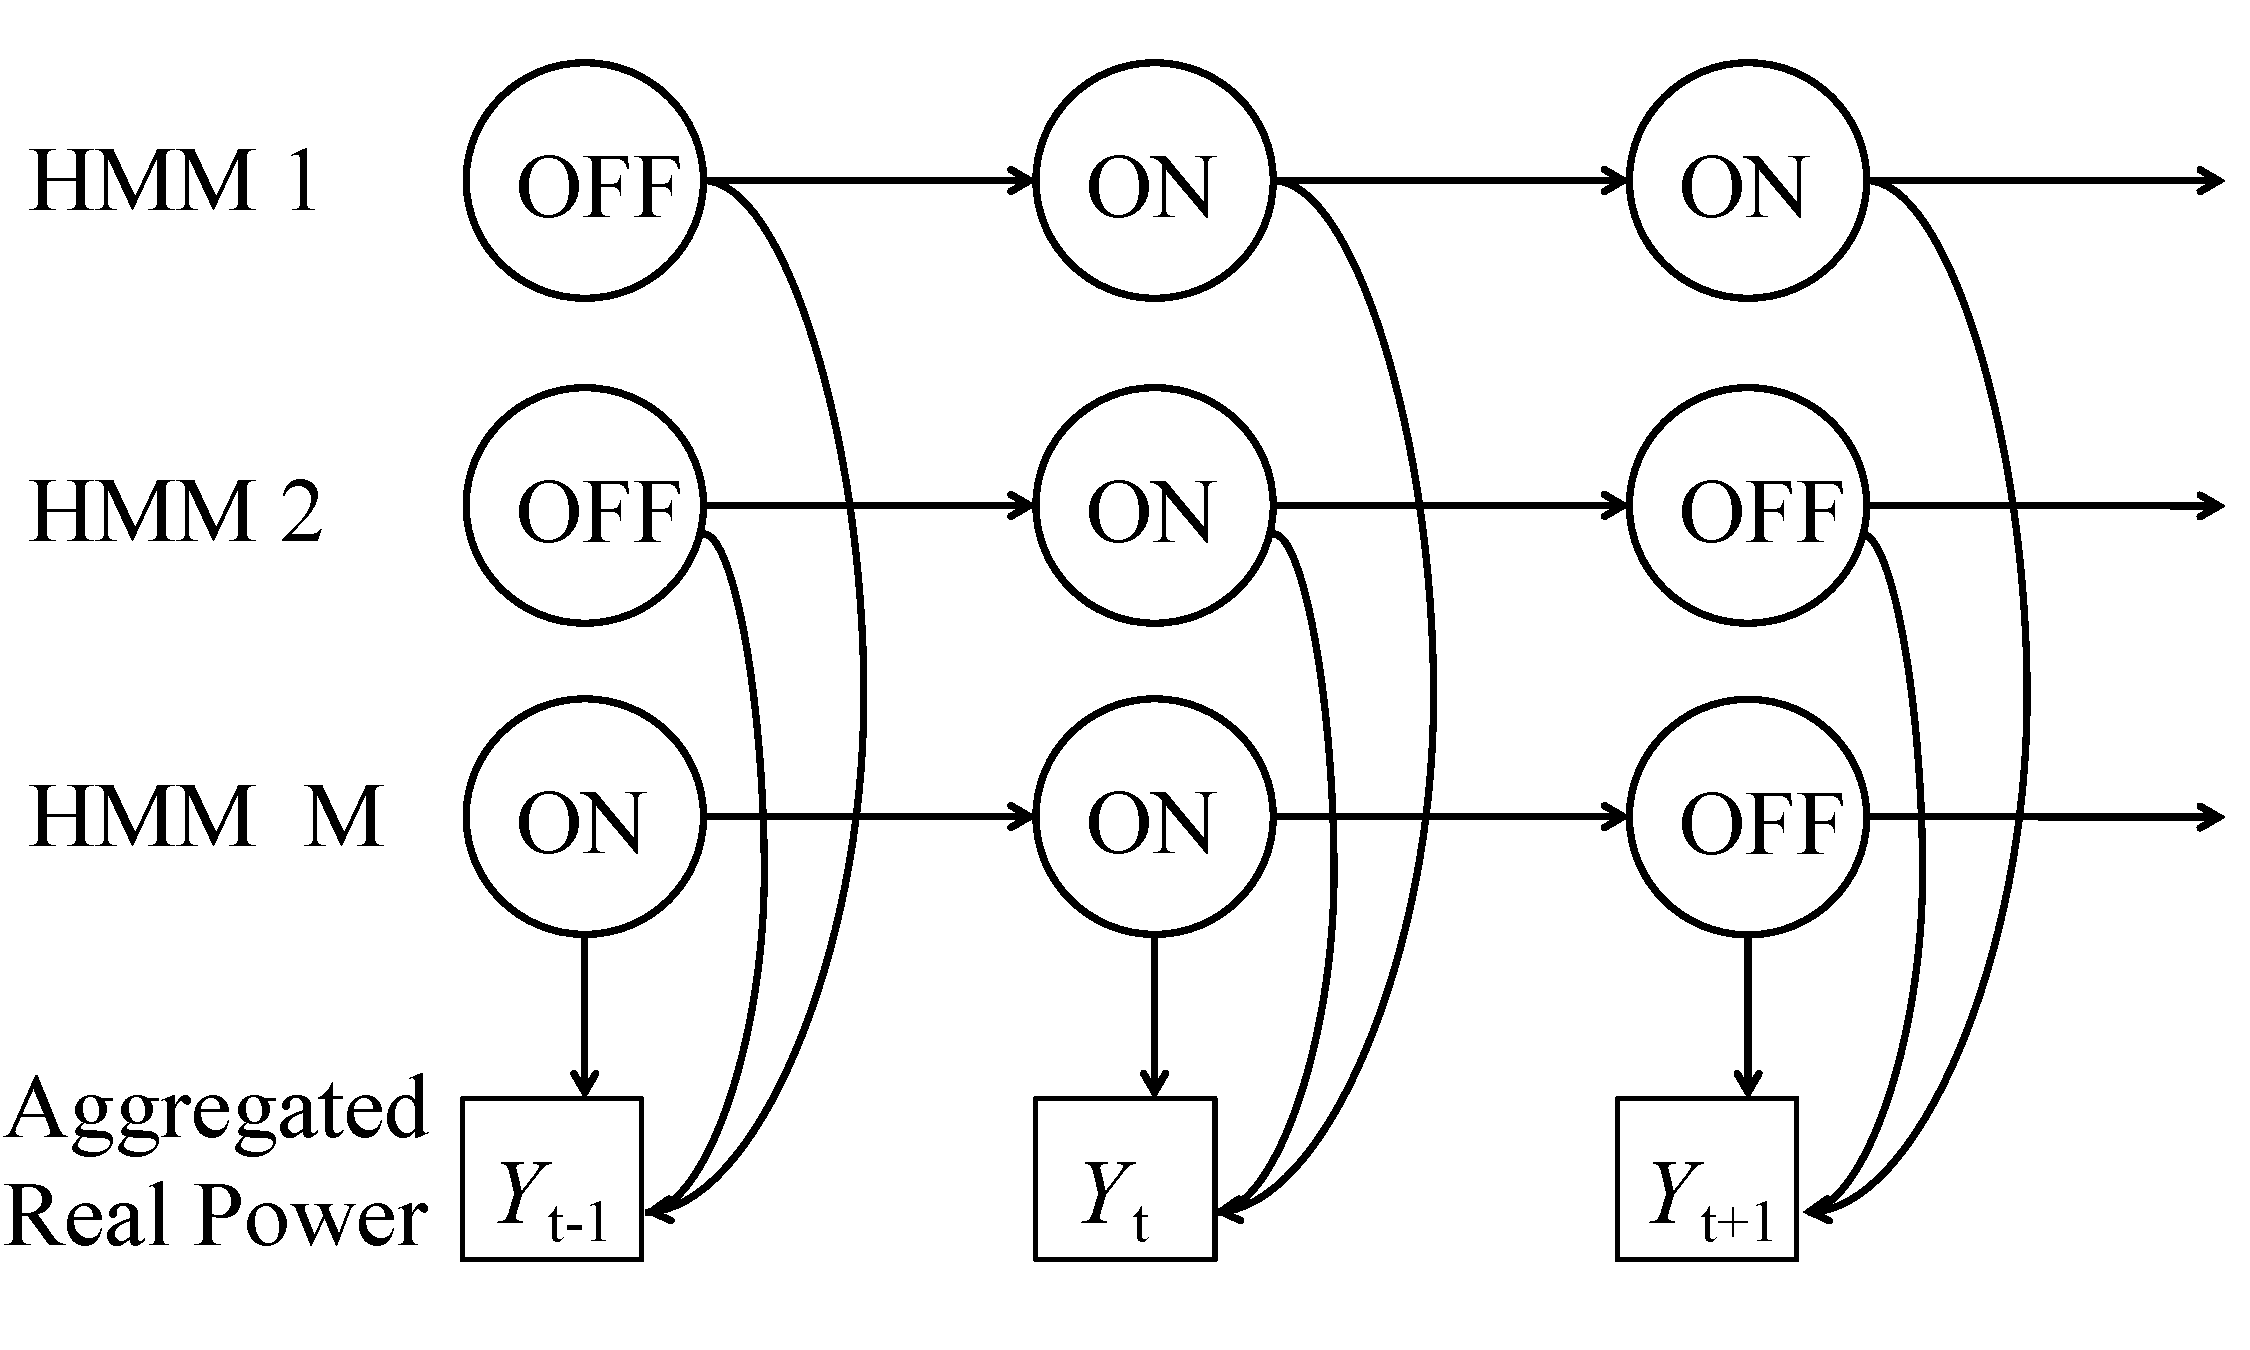
\includegraphics[width=0.5\textwidth]{figs/fhmm.pdf}\hspace{1em}&
	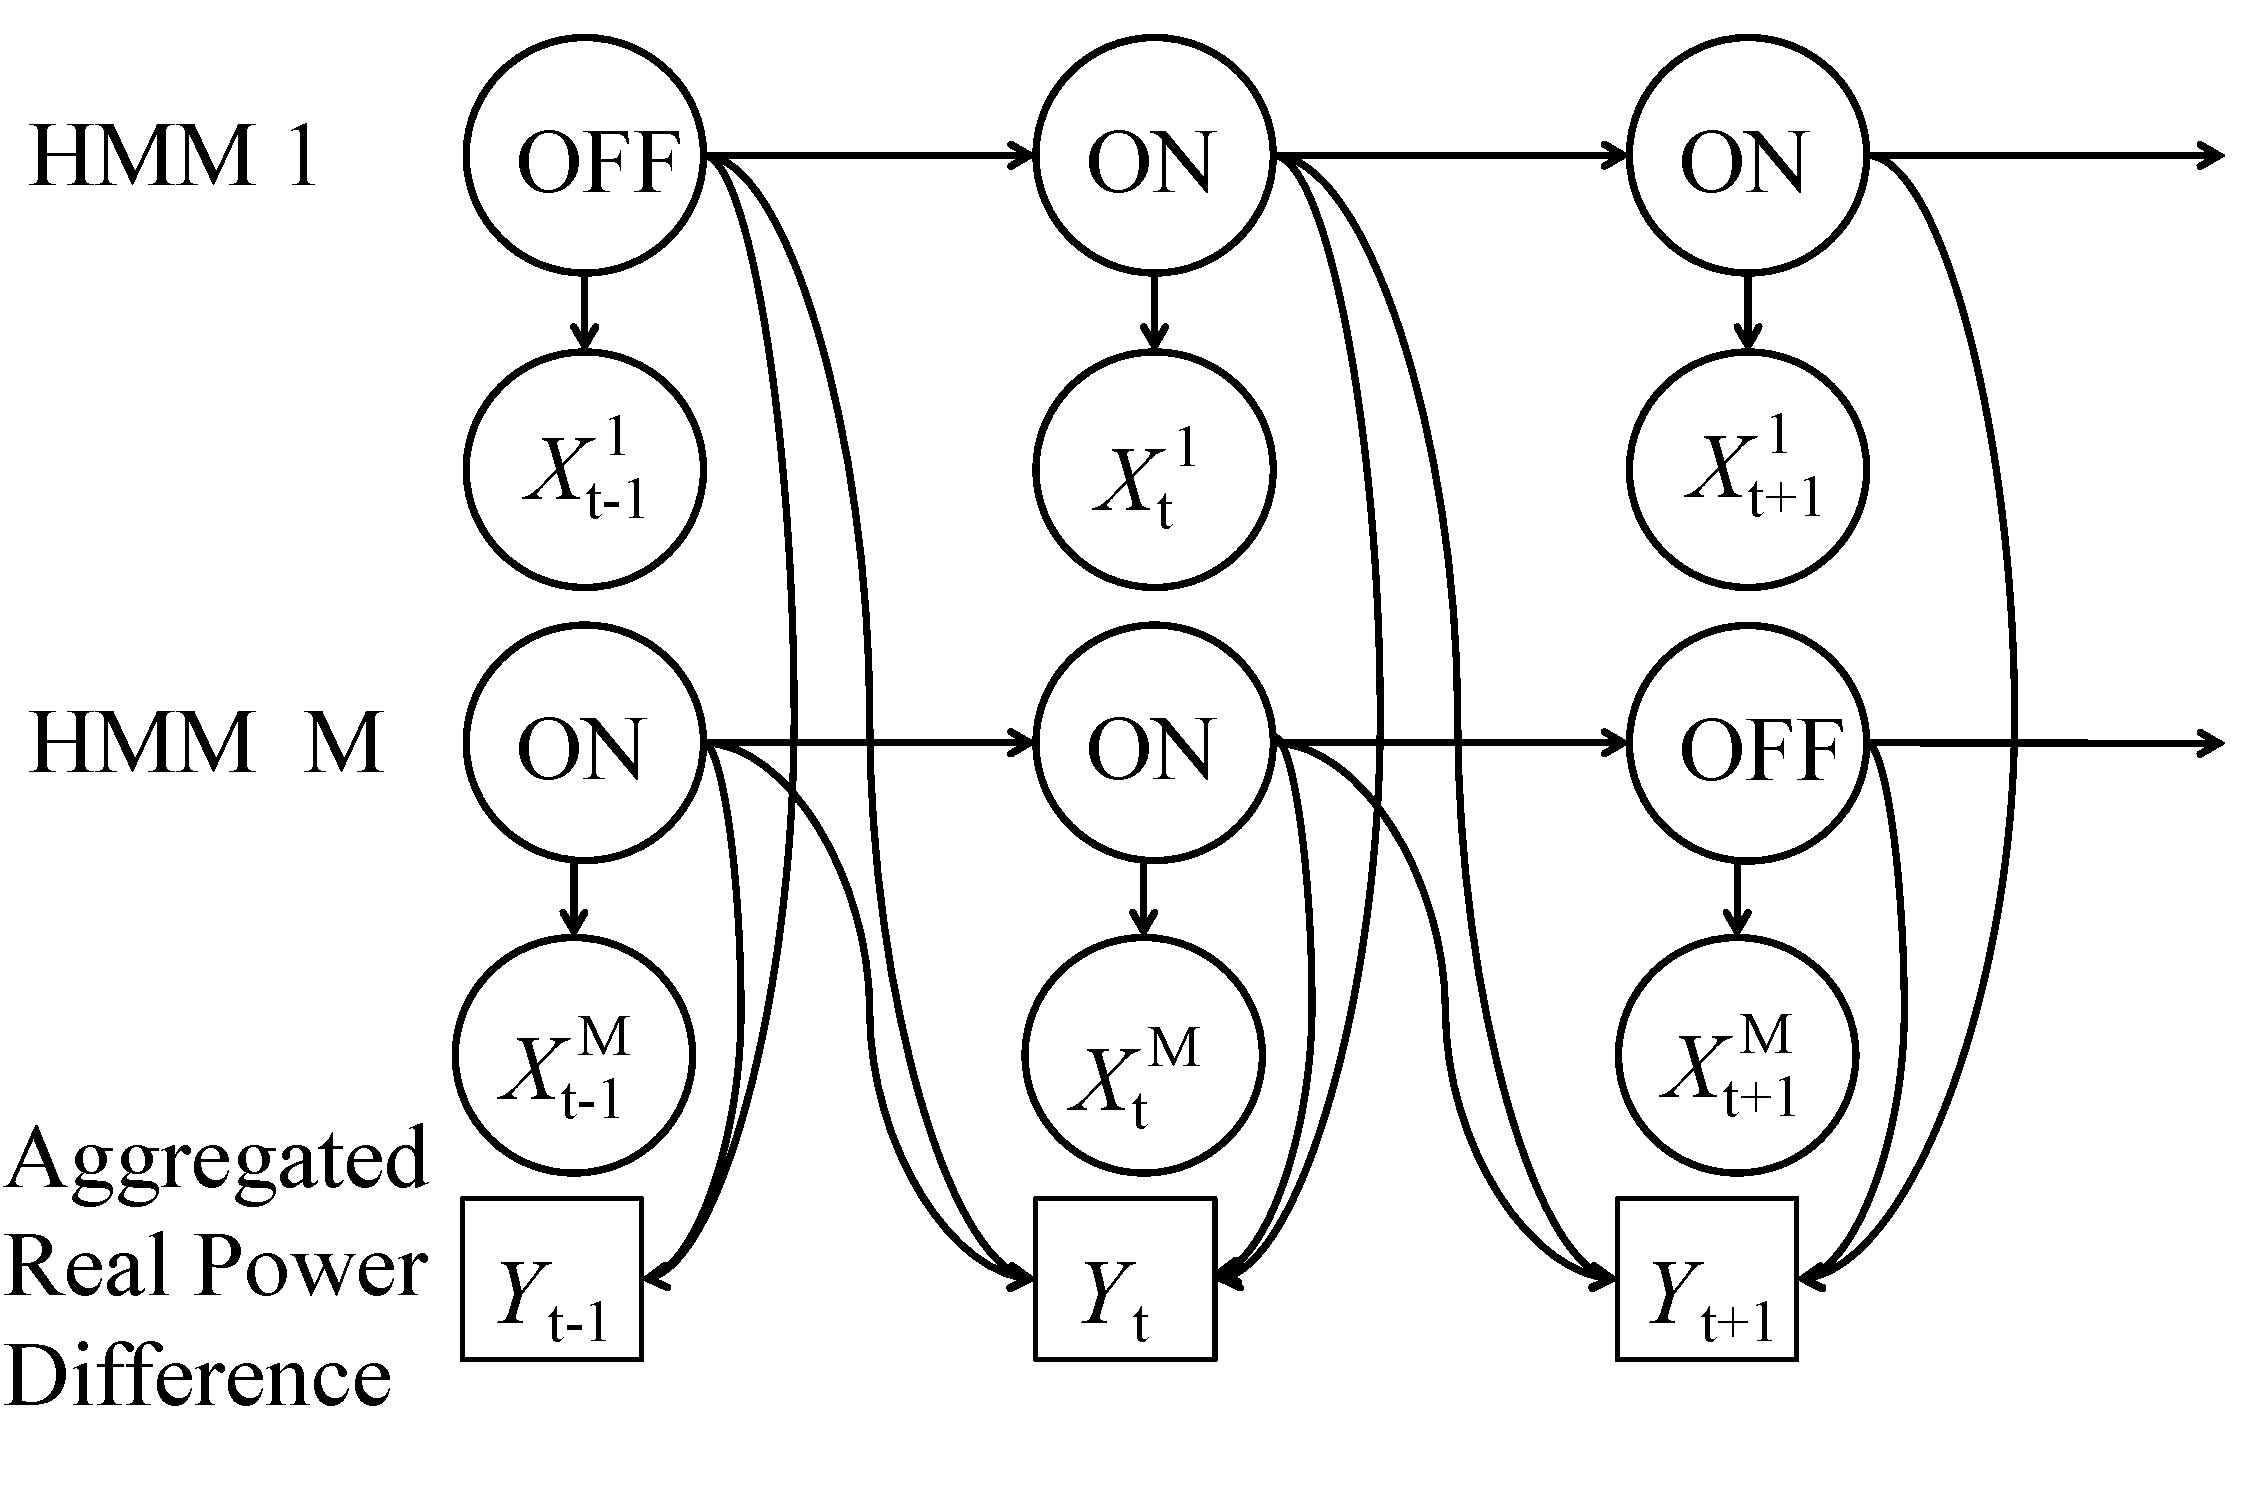
\includegraphics[width=0.5\textwidth]{figs/difference_fhmm.pdf}\tabularnewline
   (a) & (b) \tabularnewline
    \end{tabular}
    }
	\caption{ Graphical model with $M$ devices. (a) FHMM and (b) Difference FHMM.}
	\label{fig_fhmm}
\end{figure*}

FHMM and constraint FHMM
extend FHMM by incorporating the time duration for which the device is turned on, the
correlation between various devices, and the usage time of each device. 

We form the FHMM by calculating the initial probability $\phi_{in}(y,x|\Theta)$,
emission probability $\phi_{e}(y,x|\Theta)$, and
transition probability $\phi_{t}(y,x|\Theta)$,
where $\Theta$ is the parameter set.
The product of these three probability is given in Equation (\ref{eq_fhmm}).
\begin{equation}
\label{eq_fhmm}
P(y,x|\Theta)= \phi_{in}(y,x|\Theta) \cdot \phi_{e}(y,x|\Theta) \cdot \phi_{t}(y,x|\Theta)
\end{equation}
By maximizing Equation (\ref{eq_fhmm_em}) with the EM algorithm,
we can derive the HMM which represents the device. 
\begin{equation}
\label{eq_fhmm_em}
\phi(\Theta,\Theta^\prime)= \sum_x P(y,x|\Theta^\prime) log P(y,x|\Theta)
\end{equation}
where $\Theta^\prime $ and $\Theta$ represent the previous and current
iteration parameter set of the EM algorithm.

A variant of FHMM is the Additive Factorial Approximate Maximum a Posterior (AFAMAP)~\cite{kolter2012aistat}.
It is a mixture of the additive factorial model and
difference FHMM model.
The box diagram of AFAMAP is as Figure~\ref{fig_AFAMAP_boxDiagram}.
\begin{figure}[h]
\centering
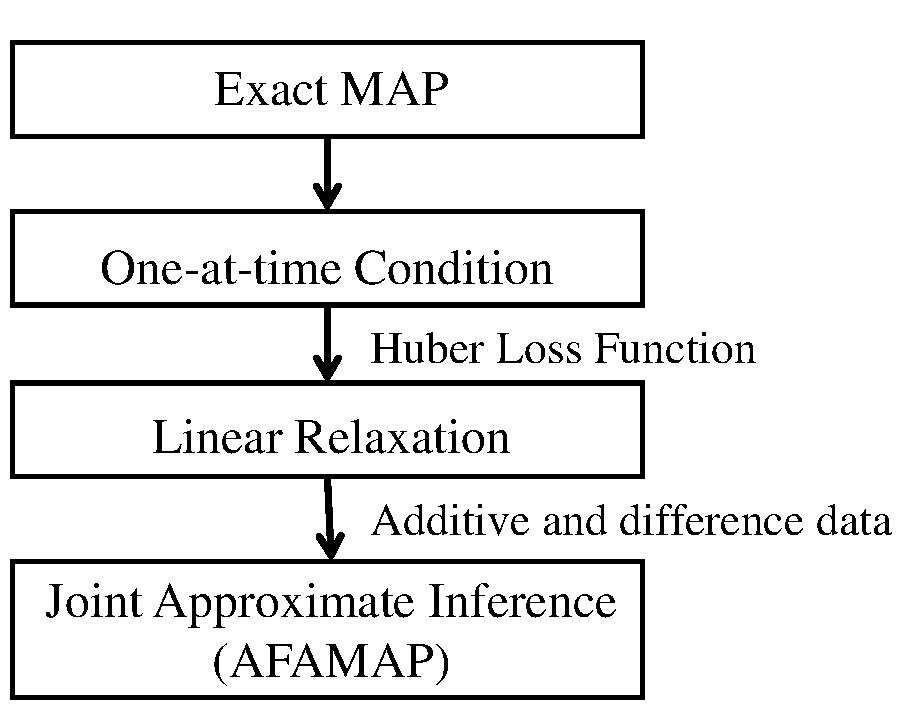
\includegraphics[width=2.5 in]{figs/AFAMAP_Boxdiagram.pdf}
\caption{AFAMAP Flowchart.}
\label{fig_AFAMAP_boxDiagram}
\end{figure}


The disaggregation procedure comprises of the following four steps. 
Initially, the MAP is proposed and
priors are defined as a Laplace prior given in Equation (\ref{eq_afamapPrior}).
\begin{equation}
\label{eq_afamapPrior}
\begin{aligned}
p(z_{1:T})= \frac{1}{Z(\theta,T)}exp\{-\theta \sum_{t=1}^{T-1} \lVert z_{t+1}-z_{t-1}\rVert_1\} \\
p(\Delta z_{1:T})=\frac{1}{Z(\theta,T)}exp\{-\theta \sum_{t=1}^{T}\lVert \Delta z_t \rVert_1\}
\end{aligned}
\end{equation}
where $z_t$ is a introduced signal, and $\Delta z_t = z_{t+1}-z_{t-1}$.
Thus the posterior of additive and difference model turns into a Gaussian distribution 
separately. 
\begin{equation}
\begin{aligned}
y_t|x_t^{(1:M)},z_t\sim \mathcal{N}(\sum_{m=1}^{M}\mu_{x_t^{(m)}}^{(m)}+\Sigma^{1/2}{z_t},\Sigma)\\
\Delta y_t|x_{t-1}^{(1:M)},\Delta z_t\sim \mathcal{N}(\sum_{m=1}^{M}\Delta \mu^{(m)}_{x_t^{(m)},x_{t-1}^{(m)}}+\Sigma^{1/2}\Delta z_t,\Sigma)\\
\end{aligned}
\end{equation}
where $\mu_j^m$ is the mean of the $m$th HMM for the state $j$, 
$x_t^{(m)} \in {1,...,S_m}$ denotes the state of the $m$th HMM at time $t$. 

Then in the second step, the once-at-a-time constraints are added as in Equation (\ref{eq_onceatime}) to limit that at any given time, 
only one device is turned on or off. 
\begin{equation}
\label{eq_onceatime}
\mathcal{O} = {\mathcal{Q}: \sum_{m,j,k \neq j} Q(x_{t-1}^{(m)},x_t^{(m)})_{j,k}\leq 1}
\end{equation}
Till this step, to solve the MAP, the computation cost is very high. 
In order to get a resolved solution, in the third step, the Huber loss function is employed to perform optimization by linear relaxation. 
\begin{equation}
\begin{aligned}
D(y,\theta)= \min_{z}\{\lVert y-z \rVert_2^2+ \theta \lVert z \rVert_1\} \\
= \sum_{\ell=1}^{n}\min\{\frac{1}{2}y_{\ell}^2,max\{\theta|y_{\ell}|-\frac{\theta^2}{2}, \frac{\theta^2}{2}\}\}
\end{aligned}
\end{equation}

Thus disaggregation is converted to a joint approximate inference AFAMAP problem.  
It's a convex quadratic program which can be solved by classical optimization algorithms.
Then with aggregated data as input, we can get the $M$ number of HMMs corresponding to $M$ devices. 

Another variant of FHMM was proposed in~\cite{parson2012nonintrusive}. 
The difference FHMM is shown as Figure~\ref{fig_fhmm} (b). 
This method assumes that we know the labels of each device, thus meaning that the number of devices and device names are known. 
However, the power usage of each device is unknown. 
In the first step, the aggregated data is 
trained to get the features of each device. 
Since this training process only uses the aggregated data, we classify this approach into unsupervised disaggregation. 
During the procedure, 
the features are repeatedly deleted. 
Then more device features are gradually identified. 
In the next step, the appliance behavior like peaks arising from device being turned on or the power demand of the device, 
obtained from the previous step is used as a prior for the difference FHMM. Then the EM algorithm is used to evaluate the likelihood of whether the profile is of a certain device type.
\begin{displaymath}
accept(y_{t},...,y_{t+w}|\hat{\theta})= \left \{ \begin{array} {ll}
true & \textrm{if $\ln\mathcal{L} > \mathcal{D}$ } \\
false & \textrm{otherwise} \end{array} \right.
\end{displaymath}
where $y_t,...,y_{t+w}$ represents the data in a window size $w$
beginning from index $t$ to $t+w$, $\mathcal{L}$ denotes the
likelihood given the prior parameter $\hat{\theta}$,
$\mathcal{D}$ is the predefined likelihood threshold.
In the final step, all these devices are disaggregated by an extended viterbi algorithm. 

Further,~\cite{huang2013designing} uses HMM for electric heat usage disaggregation. %(maybe more explanation.?)
HMM and AFAMAP are also run by additional applications~\cite{lukaszewski2013methods}. 

\textbf{Computational Complexity}
The computational cost varies for these two kinds of unsupervised learning 
approaches.
Generally the computational cost of FHMM and its variants is exponential in 
the number of latent chains.  
Theoretically, the computational complexity is 
$O(MS^{2K})$, where $M$ devices correspond to $M$ chains, 
each device has $S$ states, and $K$ latent variables~\cite{bishop2006pattern}. 
It's hard to obtain the direct solution theoretically. 
Therefore Gibbs sampling is applied to the first 
FHMM solution~\cite{kim2011unsupervised}. 
Later in the AFAMAP, QP problem techniques are used in the solution.
In another variant of difference FHMM~\cite{parson2012nonintrusive}, 
the viterbi algorithm is applied. 

\textbf{Advantages and Disadvantages of FHMM-based Unsupervised Techniques}
%The advantages and disadvantages of FHMM based unsupervised learning techniques are as follows:

The \textit{advantages} of FHMM-based unsupervised learning techniques are as follows:
\begin{enumerate}
\item It's the first formally proposed unsupervised learning approach.
\item It's solvable by introducing MCMC or converting it to an optimization problem.
\end{enumerate}

The \textit{disadvantages} of FHMM-based techniques are as below:
\begin{enumerate}
\item The computational cost is high. 
\item The parameters obtained from the MCMC approach are not easy to estimate. 
\end{enumerate}

\subsubsection{Temporal mining-based}

A lightweight time series motif mining method~\cite{shao2012temporal}
is proposed to identify devices rapidly.
In this approach, a motif which represents a multiple-state device,
is discovered in a time series of aggregated real power. 
Figure~\ref{fig_motifSample} illustrates how a motif is found.
Non-overlap search for a single episode explains
multiple-state changes for a device. A device turns on, then
its state changes to another state, until it turns off. 
This episode
corresponds to a complete running cycle of a device. A
device may include multiple episodes.
Between any two episodes, overlap does exist. For example,
the second instance of Episode1 overlaps with the first
instance of Episode 2. The overlap between episodes explains
the operations of several devices. We regard Episode
1 as device A and Episode 2 as device B. When device
B turns on for the first time, before it turns off, device A
turns on for the second time then turns off, then device B
turns off.
\begin{figure}[ht]
\centering
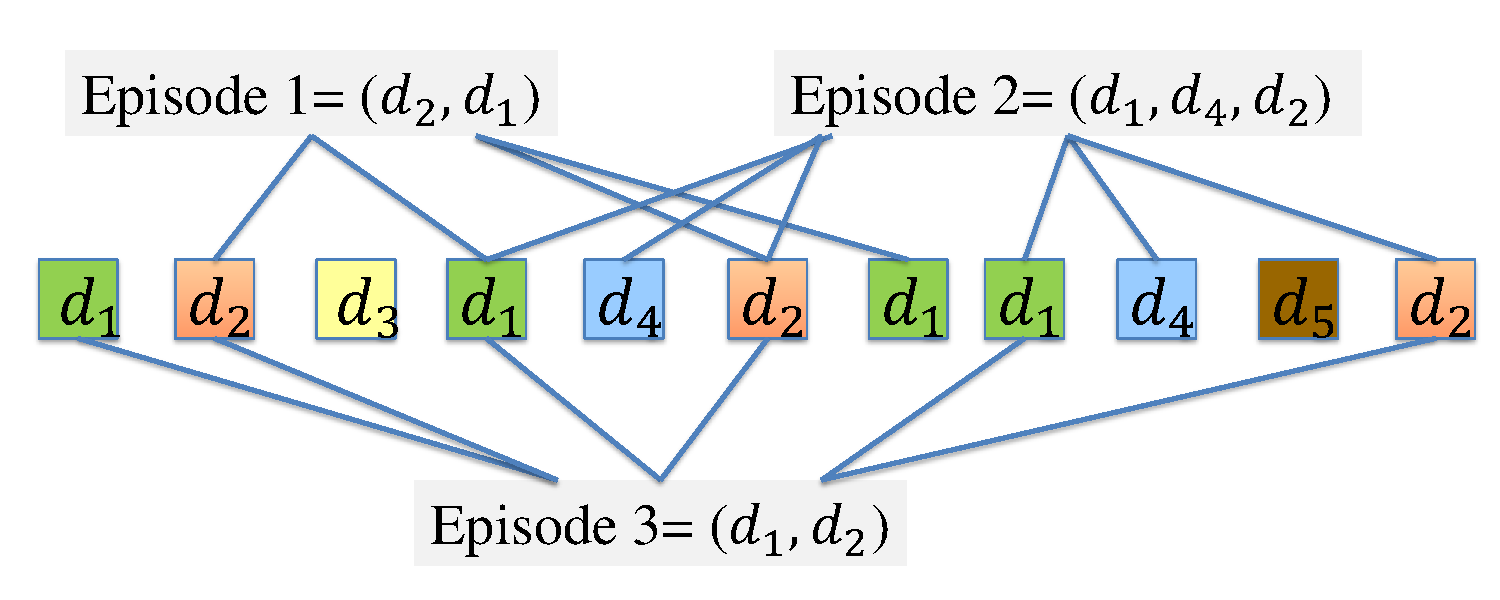
\includegraphics[width=3in]{figs/motifSample.pdf}
\caption{Motif Mining Example (\cite{shao2012temporal}). }
\label{fig_motifSample}
\end{figure}
Also, it can integrate with AFAMAP~\cite{kolter2012aistat}.
The output of motif mining can be used as the input of
AFAMAP.

\textbf{Computational Complexity}
Assume $m$ is
the number of power levels in the `diffs' data. Then the computational complexity of
DPGMM is $O(mnd^2+md^3)$, where $n$ is the number of points in diffs data,
and $d$ is the number of feature dimensions (e.g.,  time, date).
The computational complexity
for the episode generation step is $(p-1)O(m^2)$, where $p$ is the
maximal
episodes length. Since $p$, which is 3, and $m$, which is 14 or 27, are small,
we apply a brute force approach. The worst-case time complexity of the motif
mining algorithm is $O(msq)$, where $q$ is number of candidate episodes, and
$s$ is the size of the episode.

\textbf{Advantages and Disadvantages of Temporal Mining-based Unsupervised Techniques}
%The advantages and disadvantages of factorial-HMM based unsupervised learning techniques are as follows:

The \textit{advantages} of temporal mining-based techniques are as follows:
\begin{enumerate}
\item It's a lightweight approach. 
\item The disaggregation results are comparable to the results from 
complex models. 
\item It's applied to multi-state devices. 
\item It can capture device disaggregation even from commercial buildings. 
\end{enumerate}


The \textit{disadvantages} of temporal mining-based techniques are as below:
\begin{enumerate}
\item The smoothing parameter is not adjusted automatically. 
\item The problem is not formally proposed.  
\end{enumerate}

\iffalse
\subsubsection{Nonnegative matrix factor 2-D deconvolution}
A shift-invariant sparse coding model is adopted for single channel blind source separation 
in the area of signal processing~\cite{blumensath2005shift} although 
the energy dataset has not been tested so far. 
At first, the single blind source separation is formulated as a linear mixture model incorporating 
two constraints, namely sparseness and non-negativity. 
\begin{equation}
Y= XS+\epsilon
\end{equation}
Where $Y$ is the aggregated data, 
$X$ represents the feature, 
$S$ is the power level, i.e. the scalar of feature, 
and $\epsilon$ is a vector of i.i.d. Gaussian noise. 

Then three sub-problems are addressed. First is to learn the model parameters. 
The second is to infer the model states and the last is to discover the features. 
In the first step, the single source separation problem is formulated as a Bayesian problem. 
Since there are i.i.d. noise conforming to Gaussian distribution, 
$p(\epsilon) \sim N(0, \sigma_{\epsilon}I)$, 
the Gaussian likelihood is defined as $p(y|X, S) \sim N(XS, \sigma_{\epsilon}I)$. 
Take the gradient, 
$p({Y}|X) \propto \int p(Y|X, S) p(S) dS$, where $p(S)$ is the prior. 
To maximize the marginal likelihood, 
a stochastic gradient descent optimization approach is proposed by 
integrating with Monte Carlo approach. 
The features are discovered by clustering approach. 

\subsubsection{ICA or PCA-based}
\cite{davies2007source} uses ICA for signal source separation although 
the energy datasets haven't been tested yet. 

\cite{smaragdis2006probabilistic} uses the PLCA for single source separation based on 
both the time and frequency domain.
The features can be learned unsupervised by EM algorithms.
\fi

\subsubsection{Probabilistic graph-based}
Besides HMM, another probabilistic graph model was proposed by~\cite{kelly2012disaggregating}. 
The model is composed of three layers. The component layer forms the the bottom most layer, 
the second layer comprises of a probabilistic graph model that captures appliances, and
finally the top-most later us an inter-appliance layer. 
So far, this approach has not implemented in detail. 


\subsection{Semi-supervised Learning Algorithms}
Semi-supervised algorithms assume that the feature for each device, such as the power levels of 
the device is already known.
Instead of extracting features from the training data, 
it utilizes the features from the aggregated data using unsupervised algorithms. 
Then these features are used to predict devices from the test data. 

Assumption: \textit{The features are clustered based on the device i.e. all the known features
that characterize a device are grouped together.} 

\subsubsection{Clustering-based} 
Lam et al. initially propose to utilize voltage-current (V-I) trajectory of appliance as 
a feature to perform clustering~\cite{lam2007novel}.  
Hierarchical clustering are exploited to cluster the appliances by
analyzing these V-I trajectories.
When hierarchical clustering is employed,
pairwise differences between V-I's shape features
are calculated.
Then a dendrogram is created to show the
relationship between devices. % like Figure\ref{fig_dendrogram_lam2007novel}.\input{figs/unsupervised_dendrogram.tex}


\subsubsection{HMM-based}
When FHMM is proposed by~\cite{kim2011unsupervised}, 
it applies a semi-supervised learning model by integrating 
the duration when a device is turned on and off. 
Based on these durations, a semi-Markov model variant hierarchical Dirichlet 
process hidden semi Markov model (HDP-HSMM)~\cite{johnson2012bayesian} 
is adopted by extending a Bayesian nonparametric approach to capture the 
duration distribution of each device. 
 
\subsubsection{Optimization-based}
\cite{wytock2014contextually} proposes a contextual supervision approach to 
solve the single-channel source separation problem as an optimization problem. 
It uses the power levels and time of turning on and off for each device as features. 
then
\begin{equation}
\begin{aligned}
\min_{x_1,...,x_M, \theta_1, ..., \theta_M} \sum_{m=1}^{M} \{ \ell_m(x_m, Z_m\theta_m)+g_m(x_m) \} \\
s.t. \sum_{m=1}^{M}x_m=y
\end{aligned}
\end{equation}

Where $\ell_m$ and $g_m$ are loss function and regularization term related to a device $m$. 
Choose these two as convex functions then the disaggregation problem 
transforms into an optimization problem. 
Note that different $\ell$ functions are chosen for different types of device. 
$\ell_1$ norm is proper for sharp transition devices such as air conditioning. 
$\ell_2$ loss is appropriate for groups of devices with smoother dynamics. 
When we use mean average error to evaluate the performance of the methods, the results show 
that contextually supervised approach performs better than the nonnegative sparse coding. 

%don't know the computational complexity, so delete it 08/10/2015
%\textbf{Computational Complexity}
%The computational cost for contextually supervised approach is ....
%\manishc{missing text}
\textbf{Advantages and Disadvantages of Semi-unsupervised Techniques}
The advantages and disadvantages of semi-supervised learning techniques are as follows.

The \textit{advantages} of semi-supervised learning techniques are as follows:
\begin{enumerate}
\item It either learns features of each device by learning from some period's data or the feature of each device is given directly. 
\item It can disaggregate the devices more accurately than unsupervised learning, 
which knows nothing about the exact features of each device. 
\end{enumerate}


The \textit{disadvantages} of semi-supervised learning techniques are given below:
\begin{enumerate}
\item The existing features of each device are hard to be obtained. 
\item The non-parametric approach works but the computational cost is still high.
\end{enumerate}


%\cite{bellala2011towards} utilizes a semi-supervised approach on dataset from commercial buildings.

%\subsection{Non-event and Event-based}
%For these algorithms, some are related to temporal time series,
%some are only based on the events.
%Time series algorithms usually relates to the transient events or high
%frequency data involving in time and frequency.
%
%The non-event algorithms, as a function of time,
%include \citeNP{shaw2000PhdThesis,onoda2000applying,baranski2003nonintrusive,baranski2004genetic,patel2007flick,yang2007design,lam2007novel,chang2008load,chang2008load2,berges2009learning,kim2011unsupervised,liang2010load,chang2010newmethod,froehlich2011disaggregated,zeifman2011viterbi,kolter2012aistat,zeifman2012disaggregation,shao2012temporal,parson2012nonintrusive}.
%
%A variance of temporal mining is after the Fourier transform, as a function of frequency, e.g. harmonics,
%in the frequency domain \citeNP{duan2004neural,srinivasan2006neural,onoda2000applying}.
%
%The event-based algorithms include \citeNP{hart1992,roos1994using,nakano2007non,suzuki2008nonintrusive,gupta2010electrisense,berges2010enhancing,kolter2010sparse,gonccalves2011unsupervised,hampden2012closure}




